% Rapport du projet « Pronostic de défaillance de roulements » (FEMTO-ST / PRONOSTIA).
% Compiler avec XeLaTeX (Overleaf : Menu > Compilateur > XeLaTeX ; le fichier .latexmkrc le fait déjà).
% pdfLaTeX fonctionne aussi : le résumé arabe est alors inclus comme image.
% Les noms de l'équipe et les métadonnées sont dans chapitres/00_titre.tex.
\documentclass[12pt,a4paper,oneside]{report}

% ---------- polices et langues ----------
\usepackage{iftex}
\usepackage{amsmath,amssymb}
\ifXeTeX
  \usepackage{mathptmx}
  \usepackage{fontspec}
  % TeX Gyre Termes (clone libre de Times, présent dans toutes les distributions) : même rendu partout
  \setmainfont{texgyretermes}[Extension=.otf,UprightFont=*-regular,BoldFont=*-bold,
                              ItalicFont=*-italic,BoldItalicFont=*-bolditalic]
  \usepackage[bidi=default,english,french]{babel}
  \frenchsetup{StandardLists=true,SmallCapsFigTabCaptions=false}
  \babelprovide[import]{arabic}
  \babelfont[arabic]{rm}[Path=polices/,Extension=.ttf,UprightFont=*-Regular,BoldFont=*-Bold,Scale=1.12]{Amiri}
  \newcommand{\resumearabe}{\begin{otherlanguage}{arabic}\noindent{\large\bfseries ملخص}\par\medskip

يقدّم هذا التقرير دراسة مقارنة لتنبّؤ أعطال المحامل الدوّارة اعتمادًا على البيانات الحقيقية لمنصّة PRONOSTIA (معهد FEMTO-ST، تحدّي IEEE PHM 2012). تتبع موثوقية مجموعة المحامل، المقدَّرة بطريقة الإمكان الأعظم مع مراعاة البيانات المبتورة، قانون فايبل ($\beta = 1{,}85$): B10 = 125 دقيقة وB50 = 346 دقيقة، مع مجالات ثقة واسعة. يُكتشف أوّل عيب بقاعدة الثلاثة انحرافات معيارية قبل العطل بـ 7,8 دقائق في المتوسّط الوسيط، ويُبنى مؤشّر للحالة الصحّية من طاقات حزم التحويل المويجي. تُقارَن سبع طرق لتقدير العمر المتبقّي: عملية فينر البايزية هي الأدقّ (جذر متوسّط مربّع الخطأ 16,4 دقيقة) وشبكة LSTM هي الأكثر حذرًا. وتؤكّد الاختبارات على بيانات محاكاة والاختبارات الإحصائية وتحليل قابلية التفسير صحّة المنهجية. وأخيرًا، تخفّض الصيانة التنبّؤية المعتمدة على نموذج فينر كلفة الساعة بنسبة 47 ٪ مقارنةً بالصيانة التصحيحية.

\textbf{الكلمات المفاتيح:} الموثوقية، قانون فايبل، الإمكان الأعظم، العمر المتبقّي، عملية فينر، تعلّم الآلة، الصيانة التنبّؤية.
\end{otherlanguage}}
\else
  \usepackage[T1]{fontenc}
  \usepackage[utf8]{inputenc}
  \usepackage{mathptmx}
  \IfFileExists{tgtermes.sty}{\usepackage{tgtermes}}{\renewcommand{\rmdefault}{ptm}} % même police qu'avec XeLaTeX
  \usepackage[english,french]{babel}
  \frenchsetup{StandardLists=true,SmallCapsFigTabCaptions=false}
  \newcommand{\resumearabe}{\noindent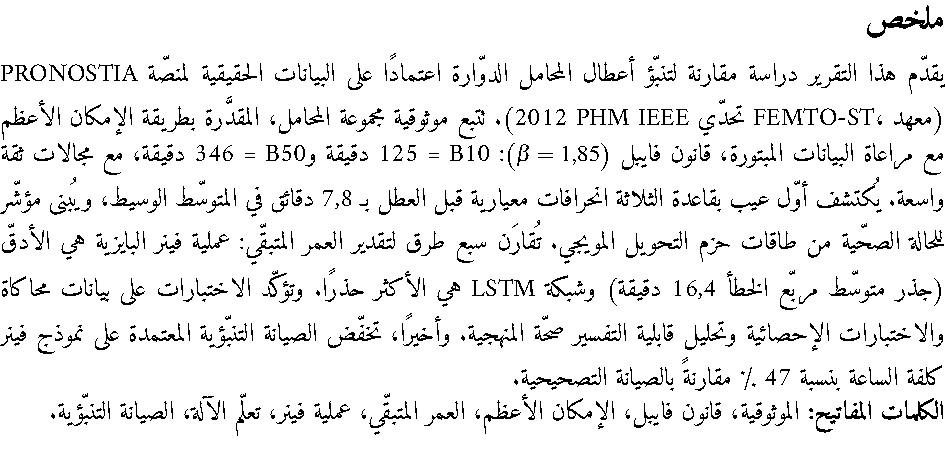
\includegraphics[width=\linewidth]{figures/resume_arabe.pdf}}
\fi

% ---------- mise en page ----------
\usepackage[a4paper,top=2.5cm,bottom=2.5cm,left=2.5cm,right=2.5cm,headheight=15pt]{geometry}
\usepackage{setspace}\setstretch{1.15}
\setlength{\parindent}{0pt}
\setlength{\parskip}{3pt}
\usepackage{xcolor}
\definecolor{terre}{RGB}{184,87,47}      % terre cuite : couleur d'accent du rapport
\definecolor{canard}{RGB}{34,116,143}    % bleu canard
\definecolor{lien}{RGB}{28,84,140}
\definecolor{gristitre}{RGB}{90,90,90}
\definecolor{fondgris}{RGB}{245,241,235}

\usepackage{titlesec}
\titleformat{\chapter}[display]{\normalfont\bfseries\fontsize{24}{28}\selectfont}
  {\chaptertitlename\ \thechapter}{12pt}{\fontsize{22}{26}\selectfont}
\titlespacing*{\chapter}{0pt}{10pt}{20pt}
\titleformat{name=\chapter,numberless}[display]{\normalfont\bfseries\fontsize{24}{28}\selectfont}{}{0pt}{}
\titlespacing*{name=\chapter,numberless}{0pt}{10pt}{20pt}
\titleformat{\section}{\normalfont\Large\bfseries\color{gristitre}}{\thesection}{0.8em}{}
\titleformat{\subsection}{\normalfont\large\bfseries\color{gristitre}}{\thesubsection}{0.8em}{}
\titlespacing*{\section}{0pt}{14pt}{6pt}
\titlespacing*{\subsection}{0pt}{10pt}{4pt}

\usepackage{fancyhdr}
\pagestyle{fancy}\fancyhf{}
\fancyhead[L]{\small\color{gristitre}Pronostic de défaillance de roulements}
\fancyhead[R]{\small\color{gristitre}\nouppercase{\leftmark}}
\fancyfoot[C]{\thepage}
\renewcommand{\headrulewidth}{0.5pt}
\renewcommand{\chaptermark}[1]{\markboth{\chaptername\ \thechapter.\ #1}{}}
\fancypagestyle{plain}{\fancyhf{}\fancyfoot[C]{\thepage}\renewcommand{\headrulewidth}{0pt}}
\newcommand{\frontmark}[1]{\markboth{#1}{#1}}

% ---------- contenu ----------
\usepackage{graphicx}
\usepackage{booktabs,tabularx,array,multirow}
\usepackage{enumitem}\setlist{itemsep=1pt,topsep=3pt}\setlist[itemize]{label=\textbullet}
\setlength{\emergencystretch}{1.5em} % évite les lignes qui dépassent dans la marge
\usepackage{caption}\captionsetup{labelsep=colon,font=small,skip=6pt}
\usepackage{float}
\usepackage{multicol}
\usepackage[most]{tcolorbox}
\usepackage{tikz}
\usetikzlibrary{positioning,arrows.meta,calc}
\usepackage[hidelinks,colorlinks=true,linkcolor=lien,citecolor=canard,urlcolor=lien]{hyperref}
\hypersetup{pdftitle={Étude comparative de pronostic de défaillance de roulements},
  pdfsubject={Projet de Sûreté de Fonctionnement et Maintenance, ENSIT, GMAM 3},
  pdfkeywords={fiabilité, Weibull, durée de vie résiduelle, processus de Wiener, PRONOSTIA}}

\newtcolorbox{encadre}{colback=fondgris,colframe=terre,boxrule=0pt,leftrule=3pt,arc=0pt,
  left=10pt,right=10pt,top=6pt,bottom=6pt}
\newcolumntype{Y}{>{\raggedright\arraybackslash}X}
\newcommand{\chapintro}{\section*{Introduction}}
\newcommand{\chapconclusion}{\section*{Conclusion}}

\addto\captionsfrench{\renewcommand{\listfigurename}{Liste des figures}\renewcommand{\listtablename}{Liste des tableaux}%
  \renewcommand{\tablename}{Tableau}\renewcommand{\contentsname}{Table des matières}\renewcommand{\bibname}{Bibliographie}}
\setcounter{tocdepth}{1}
% table des matières et listes plus compactes (pour tenir chacune sur une page)
\usepackage[titles]{tocloft}
\setlength{\cftbeforechapskip}{4pt}
\setlength{\cftbeforefigskip}{0pt}
\setlength{\cftbeforetabskip}{0pt}
\usepackage{etoolbox}
\makeatletter
\patchcmd{\@chapter}{\addtocontents{lof}{\protect\addvspace{10\p@}}}{}{}{}
\patchcmd{\@chapter}{\addtocontents{lot}{\protect\addvspace{10\p@}}}{}{}{}
\makeatother
% bibliographie sans espace entre les références
\let\anciennebiblio\thebibliography
\renewcommand{\thebibliography}[1]{\anciennebiblio{#1}\setlength{\itemsep}{0pt}\setlength{\parskip}{0pt}}

\begin{document}
% =================== PAGE DE GARDE ===================
% Pour ajouter les membres de l'équipe : modifier la ligne « \newcommand{\equipe}{...} » ci-dessous.
\newcommand{\equipe}{Farah Belghith}
\begin{titlepage}
\newgeometry{top=1.4cm,bottom=1.6cm,left=2.4cm,right=2.4cm}
\setstretch{1.05}
\centering
\noindent
\begin{minipage}[c]{0.3\linewidth}\raggedright
  
\includegraphics[height=2.1cm,keepaspectratio]{figures/logo_univ_tunis.png}
\end{minipage}%
\begin{minipage}[c]{0.4\linewidth}\centering
  
\includegraphics[height=2.2cm,keepaspectratio]{figures/logo_emblem.png}
\end{minipage}%
\begin{minipage}[c]{0.3\linewidth}\raggedleft
  
\includegraphics[height=1.5cm,keepaspectratio]{figures/logo_ensit.png}
\end{minipage}

\vspace{0.5cm}
\rule{\linewidth}{1pt}\par
\vspace{0.35cm}
{\large\bfseries UNIVERSITÉ DE TUNIS\par}
\vspace{2pt}
{\large\bfseries ÉCOLE NATIONALE SUPÉRIEURE D'INGÉNIEURS DE TUNIS\par}
\vspace{2pt}
{\bfseries DÉPARTEMENT DE GÉNIE MATHÉMATIQUE\par}
\vspace{0.3cm}
\rule{\linewidth}{1pt}\par

\vfill
{\LARGE\bfseries Projet de Sûreté de Fonctionnement et Maintenance\par}
\vspace{0.35em}
{\normalsize\bfseries Troisième année — Génie Mathématiques Appliquées et Modélisation (GMAM 3)\par}

\vspace{0.7cm}
{\normalsize Réalisé par :\par}
\vspace{0.4em}
{\LARGE\bfseries \equipe\par}

\vfill
{\color{terre}\rule{0.85\linewidth}{0.8pt}}\par
\vspace{0.7em}
{\fontsize{24}{30}\selectfont\bfseries Étude comparative de pronostic\\ de défaillance de roulements\par}
\vspace{0.5em}
{\large\bfseries Fiabilité, premier défaut, durée de vie résiduelle\\ et décision de maintenance (FEMTO-ST / PRONOSTIA)\par}
\vspace{0.7em}
{\color{terre}\rule{0.85\linewidth}{0.8pt}}\par

\vfill
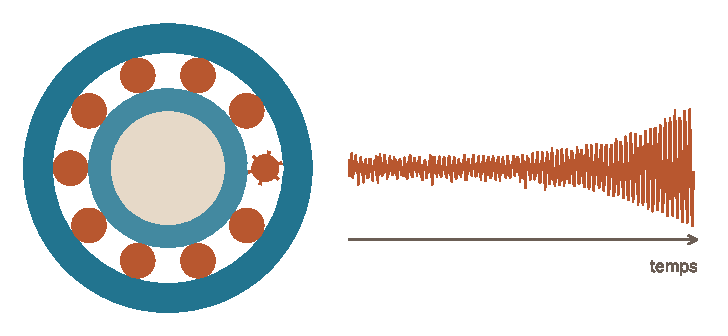
\includegraphics[height=3.9cm,keepaspectratio]{figures/illustration_couverture.pdf}\par

\vfill
{\normalsize Rapport de projet\par}
\vspace{0.5em}
{\normalsize\textbf{Encadré par :} M. Fayçal Ben Hmida\par}

\vfill
{\normalsize\textbf{Année universitaire :} 2026–2027\par}

\restoregeometry
\end{titlepage}


\pagenumbering{arabic}
\chapter*{Dédicaces}
\addcontentsline{toc}{chapter}{Dédicaces}
\frontmark{Dédicaces}

\vspace*{0.3cm}
\begin{center}
\itshape
À nos parents,\\
pour leur amour, leur patience\\
et leur soutien à chaque étape de nos études.\\[1.4em]
À nos familles et à nos amis,\\
qui ont cru en nous, même pendant les nuits de calcul.\\[1.4em]
À nos enseignants,\\
qui nous ont appris à poser les bonnes questions\\
avant de chercher les réponses.
\end{center}

\vspace{1.2cm}
{\normalfont\bfseries\fontsize{24}{28}\selectfont Remerciements\par}
\addcontentsline{toc}{chapter}{Remerciements}
\vspace{0.6cm}

Nous remercions très sincèrement \textbf{M. Fayçal Ben Hmida}, enseignant du module « Sûreté de fonctionnement et maintenance », pour la clarté de son cours, pour ses conseils pendant les séances de suivi et pour les points précis qu'il nous a demandé de traiter : ils ont guidé toute la structure de ce rapport.

Nous remercions aussi l'ensemble des enseignants de l'École Nationale Supérieure d'Ingénieurs de Tunis (ENSIT), qui nous ont donné les outils de statistique, de fiabilité et d'apprentissage automatique utilisés ici.

Merci enfin à l'institut FEMTO-ST et aux organisateurs du challenge IEEE PHM 2012, qui ont rendu publiques les données du banc PRONOSTIA, sans lesquelles ce travail n'aurait pas été possible.

{\setstretch{1.0}\small\tableofcontents}

\clearpage\frontmark{Liste des figures et des tableaux}
{\setstretch{1.0}\small
\listoffigures
\begingroup\let\clearpage\relax\vspace{-1.3cm}\listoftables\endgroup
}

\chapter*{Liste des abréviations}
\addcontentsline{toc}{chapter}{Liste des abréviations}
\frontmark{Liste des abréviations}

{\setstretch{1.05}\small\setlength{\parskip}{2.5pt}
\textbf{AFT} : modèle à temps de vie accéléré (\emph{accelerated failure time}).

\textbf{AIC} : critère d'information d'Akaike (plus petit = meilleur compromis entre précision et simplicité).

\textbf{B10, B50} : âge auquel 10 \% (resp. 50 \%) des roulements ont défailli.

\textbf{CBM} : maintenance conditionnelle (\emph{condition-based maintenance}).

\textbf{CNN 1D} : réseau de neurones à convolution sur une dimension (le temps).

\textbf{FPT} : instant du premier défaut détecté (\emph{first predicting time}).

\textbf{GPR} : régression par processus gaussien.

\textbf{HI} : indicateur de santé (\emph{health indicator}).

\textbf{IC} : intervalle de confiance.

\textbf{KPI} : indicateur clé de performance (\emph{key performance indicator}).

\textbf{L10} : durée de vie nominale des catalogues (atteinte par 90 \% des roulements).

\textbf{LSTM} : réseau de neurones récurrent à mémoire longue (\emph{long short-term memory}).

\textbf{MAE} : erreur absolue moyenne.

\textbf{MRL} : durée de vie résiduelle moyenne (\emph{mean residual life}).

\textbf{MTTF} : durée moyenne de fonctionnement avant défaillance (\emph{mean time to failure}).

\textbf{MV} : maximum de vraisemblance.

\textbf{PHM} : surveillance de la santé et pronostic (\emph{prognostics and health management}).

\textbf{RF} : forêt aléatoire (\emph{random forest}).

\textbf{RMSE} : racine de l'erreur quadratique moyenne.

\textbf{RUL} : durée de vie résiduelle (\emph{remaining useful life}).

\textbf{SVR} : régression à vecteurs de support (\emph{support vector regression}).

\textbf{XAI} : intelligence artificielle explicable (\emph{explainable AI}).
}

\clearpage
\chapter*{Introduction générale}
\addcontentsline{toc}{chapter}{Introduction générale}
\frontmark{Introduction générale}

Les roulements sont partout : moteurs, pompes, ventilateurs, réducteurs. Quand un roulement casse, la machine s'arrête, souvent sans prévenir, et la panne peut abîmer d'autres pièces. À l'inverse, le changer trop tôt revient à jeter une pièce encore bonne. Pour trouver le bon moment, il faut savoir estimer, pour chaque roulement, sa \textbf{durée de vie résiduelle} (RUL) : le temps qu'il lui reste avant la panne.

Ce projet, réalisé dans le module « Sûreté de fonctionnement et maintenance », traite cette question sur les données réelles du banc PRONOSTIA de l'institut FEMTO-ST, utilisées pour le challenge IEEE PHM 2012 \cite{nectoux2012,phm2012challenge} : 17 roulements usés jusqu'à la casse sous trois conditions de charge et de vitesse.

\begin{encadre}
\textbf{Problématique.} À partir des vibrations d'un roulement, peut-on prédire sa durée de vie résiduelle, avec quelle précision, et quelle famille de méthodes marche le mieux : la fiabilité de la population, un modèle stochastique, l'apprentissage automatique classique ou l'apprentissage profond ? Et que gagne-t-on, en coût de maintenance, à utiliser ces prédictions ?
\end{encadre}

Nous avons travaillé en quatre sprints, du signal brut jusqu'à la décision de maintenance :
\begin{enumerate}
  \item \textbf{données et fiabilité} : lecture et contrôle des 24 889 fichiers, filtrage, lois de durée de vie, B10, B50 ;
  \item \textbf{santé du roulement} : indicateurs de vibration, détection du premier défaut, indicateur de santé ;
  \item \textbf{modèles} : sept méthodes de prédiction de la RUL, réglées sans jamais regarder les roulements de test ;
  \item \textbf{évaluation et décision} : critères de jugement, tests, explicabilité et analyse économique.
\end{enumerate}

Le rapport suit cette démarche. Le chapitre 1 présente le cadre industriel, l'état de l'art et les données. Le chapitre 2 décrit la méthodologie complète, de A à Z. Le chapitre 3 donne les résultats et compare les méthodes. Le chapitre 4 transforme les prédictions en décisions de maintenance, chiffre le gain économique et propose des perspectives. Tous les résultats sont aussi présentés dans un tableau de bord interactif.

\chapter{Cadre industriel, état de l'art et données}

\chapintro
Ce chapitre situe le projet dans la maintenance industrielle, résume les méthodes de pronostic utilisées dans la littérature, puis décrit les données PRONOSTIA.

\section{Les stratégies de maintenance}

La norme NF EN 13306 \cite{nf13306} distingue trois grandes stratégies de maintenance (tableau~\ref{tab:strategies}). Notre projet relève de la maintenance \textbf{prévisionnelle} : on mesure l'état du roulement et on prévoit son évolution pour intervenir au bon moment \cite{jardine2006}.

\begin{table}[H]
\centering\small
\begin{tabularx}{\linewidth}{lYYY}
\toprule
Stratégie & Principe & Avantage & Inconvénient \\
\midrule
Corrective & on répare après la panne & rien à surveiller & arrêt imprévu, dégâts, coût élevé \\
Préventive systématique & on remplace à un âge fixé & facile à planifier & on jette des pièces encore bonnes \\
Conditionnelle et prévisionnelle & on mesure l'état et on prévoit la panne & on intervient au bon moment & capteurs, données et modèles nécessaires \\
\bottomrule
\end{tabularx}
\caption[Stratégies de maintenance (NF EN 13306)]{Les trois stratégies de maintenance (NF EN 13306).}
\label{tab:strategies}
\end{table}

\section{Cadre industriel du projet}

La norme ISO 13374 \cite{iso13374} découpe la surveillance d'une machine en six blocs de traitement. Le tableau~\ref{tab:iso} montre que notre chaîne suit ces six blocs dans l'ordre : le projet a la forme d'un vrai système industriel de surveillance, du capteur jusqu'à l'aide à la décision.

\begin{table}[H]
\centering\small
\begin{tabularx}{\linewidth}{lY}
\toprule
Bloc ISO 13374 & Dans notre projet \\
\midrule
1. Acquisition des données & 2 accéléromètres, 25,6 kHz, 0,1 s toutes les 10 s \\
2. Traitement des données & filtrage, 36 indicateurs de vibration (features) \\
3. Détection d'état & premier défaut par la règle des 3 $\sigma$ \\
4. Évaluation de la santé & indicateur de santé (HI) \\
5. Pronostic & RUL prédite par 7 méthodes, avec incertitude \\
6. Aide à la décision & quand remplacer le roulement, et combien on économise \\
\bottomrule
\end{tabularx}
\caption[Blocs de la norme ISO 13374 dans le projet]{Les six blocs de la norme ISO 13374 dans notre projet.}
\label{tab:iso}
\end{table}

\section{État de l'art}

Les méthodes de pronostic se rangent en trois familles \cite{lei2018,si2011} :
\begin{itemize}
  \item \textbf{fiabilité de la population} : une loi de durée de vie (Weibull \cite{weibull1951}) estimée sur un parc, sans capteur. Elle donne le B10 ou le MTTF, mais la même réponse pour tous les roulements ;
  \item \textbf{modèles stochastiques de dégradation} : l'indicateur de santé suit un processus aléatoire, souvent un processus de Wiener, et la RUL est le temps pour atteindre un seuil \cite{si2011,zhang2018}. Ils donnent naturellement un intervalle d'incertitude ;
  \item \textbf{modèles guidés par les données} : SVR \cite{drucker1997}, processus gaussiens \cite{rasmussen2006}, forêts aléatoires \cite{breiman2001}, puis réseaux profonds LSTM \cite{hochreiter1997} et CNN \cite{li2018cnn}, qui apprennent directement le lien entre les mesures et la RUL.
\end{itemize}
Sur PRONOSTIA, l'étude comparative récente de Dhungana et al. \cite{dhungana2025} montre que les résultats varient beaucoup d'un roulement à l'autre et que le choix de l'indicateur de santé compte autant que le modèle. Pour choisir cet indicateur, nous utilisons les critères de Coble et Hines \cite{coble2009}.

\section{Les données PRONOSTIA}

\subsection{Le banc et les conditions d'essai}
Le banc PRONOSTIA use un roulement plus vite que la normale grâce à une forte charge radiale \cite{nectoux2012}. Deux accéléromètres (horizontal et vertical) enregistrent 0,1 s de signal (2 560 points à 25,6 kHz) toutes les 10 s, et l'essai s'arrête quand la vibration dépasse 20 g. Le tableau~\ref{tab:conditions} donne les trois conditions et le découpage des roulements.

\begin{table}[H]
\centering\small
\begin{tabular}{cccll}
\toprule
Condition & Vitesse & Charge & Apprentissage (complets) & Test (arrêtés avant la fin) \\
\midrule
1 & 1 800 tr/min & 4 000 N & Bearing1\_1, Bearing1\_2 & Bearing1\_3 à Bearing1\_7 \\
2 & 1 650 tr/min & 4 200 N & Bearing2\_1, Bearing2\_2 & Bearing2\_3 à Bearing2\_7 \\
3 & 1 500 tr/min & 5 000 N & Bearing3\_1, Bearing3\_2 & Bearing3\_3 \\
\bottomrule
\end{tabular}
\caption[Conditions opératoires et découpage des roulements]{Conditions opératoires et découpage des 17 roulements.}
\label{tab:conditions}
\end{table}

\subsection{Différents types d'essais}
En fiabilité, on ne traite pas de la même façon un essai qui va jusqu'à la panne et un essai arrêté avant (tableau~\ref{tab:essais}). Les 11 roulements de test sont des \textbf{données censurées à droite} : on sait seulement qu'ils fonctionnaient encore à l'instant de troncature du challenge. L'estimateur de Kaplan-Meier \cite{kaplan1958} et le maximum de vraisemblance savent utiliser cette information.

\begin{table}[H]
\centering\small
\begin{tabularx}{\linewidth}{lYY}
\toprule
Type d'essai & Définition & Dans nos données \\
\midrule
Essai complet & on attend la panne & les 6 roulements d'apprentissage \\
Essai censuré à droite & on arrête à une date fixée à l'avance, avant la panne & les 11 roulements de test, arrêtés à la troncature \\
Essai accéléré & on use plus vite avec une charge forte & tout le banc (4 000 à 5 000 N) \\
\bottomrule
\end{tabularx}
\caption[Types d'essais présents dans les données]{Les types d'essais présents dans les données.}
\label{tab:essais}
\end{table}

\subsection{Contrôle qualité}
Aucun fichier n'est incomplet et aucune valeur ne manque. Bearing1\_1 contient 3 horodatages incohérents : le temps est reconstruit à partir du numéro du fichier (10 s par fichier). Pour Bearing1\_4, la RUL officielle (339 s) ne correspond pas au nombre de fichiers (2 890 s) : c'est une erreur connue du jeu de données, et nous gardons la valeur officielle pour le score du challenge. La figure~\ref{fig:durees} montre la grande dispersion des durées de vie : de 38 à 467 min, même sous une même condition.

\begin{figure}[H]
\centering
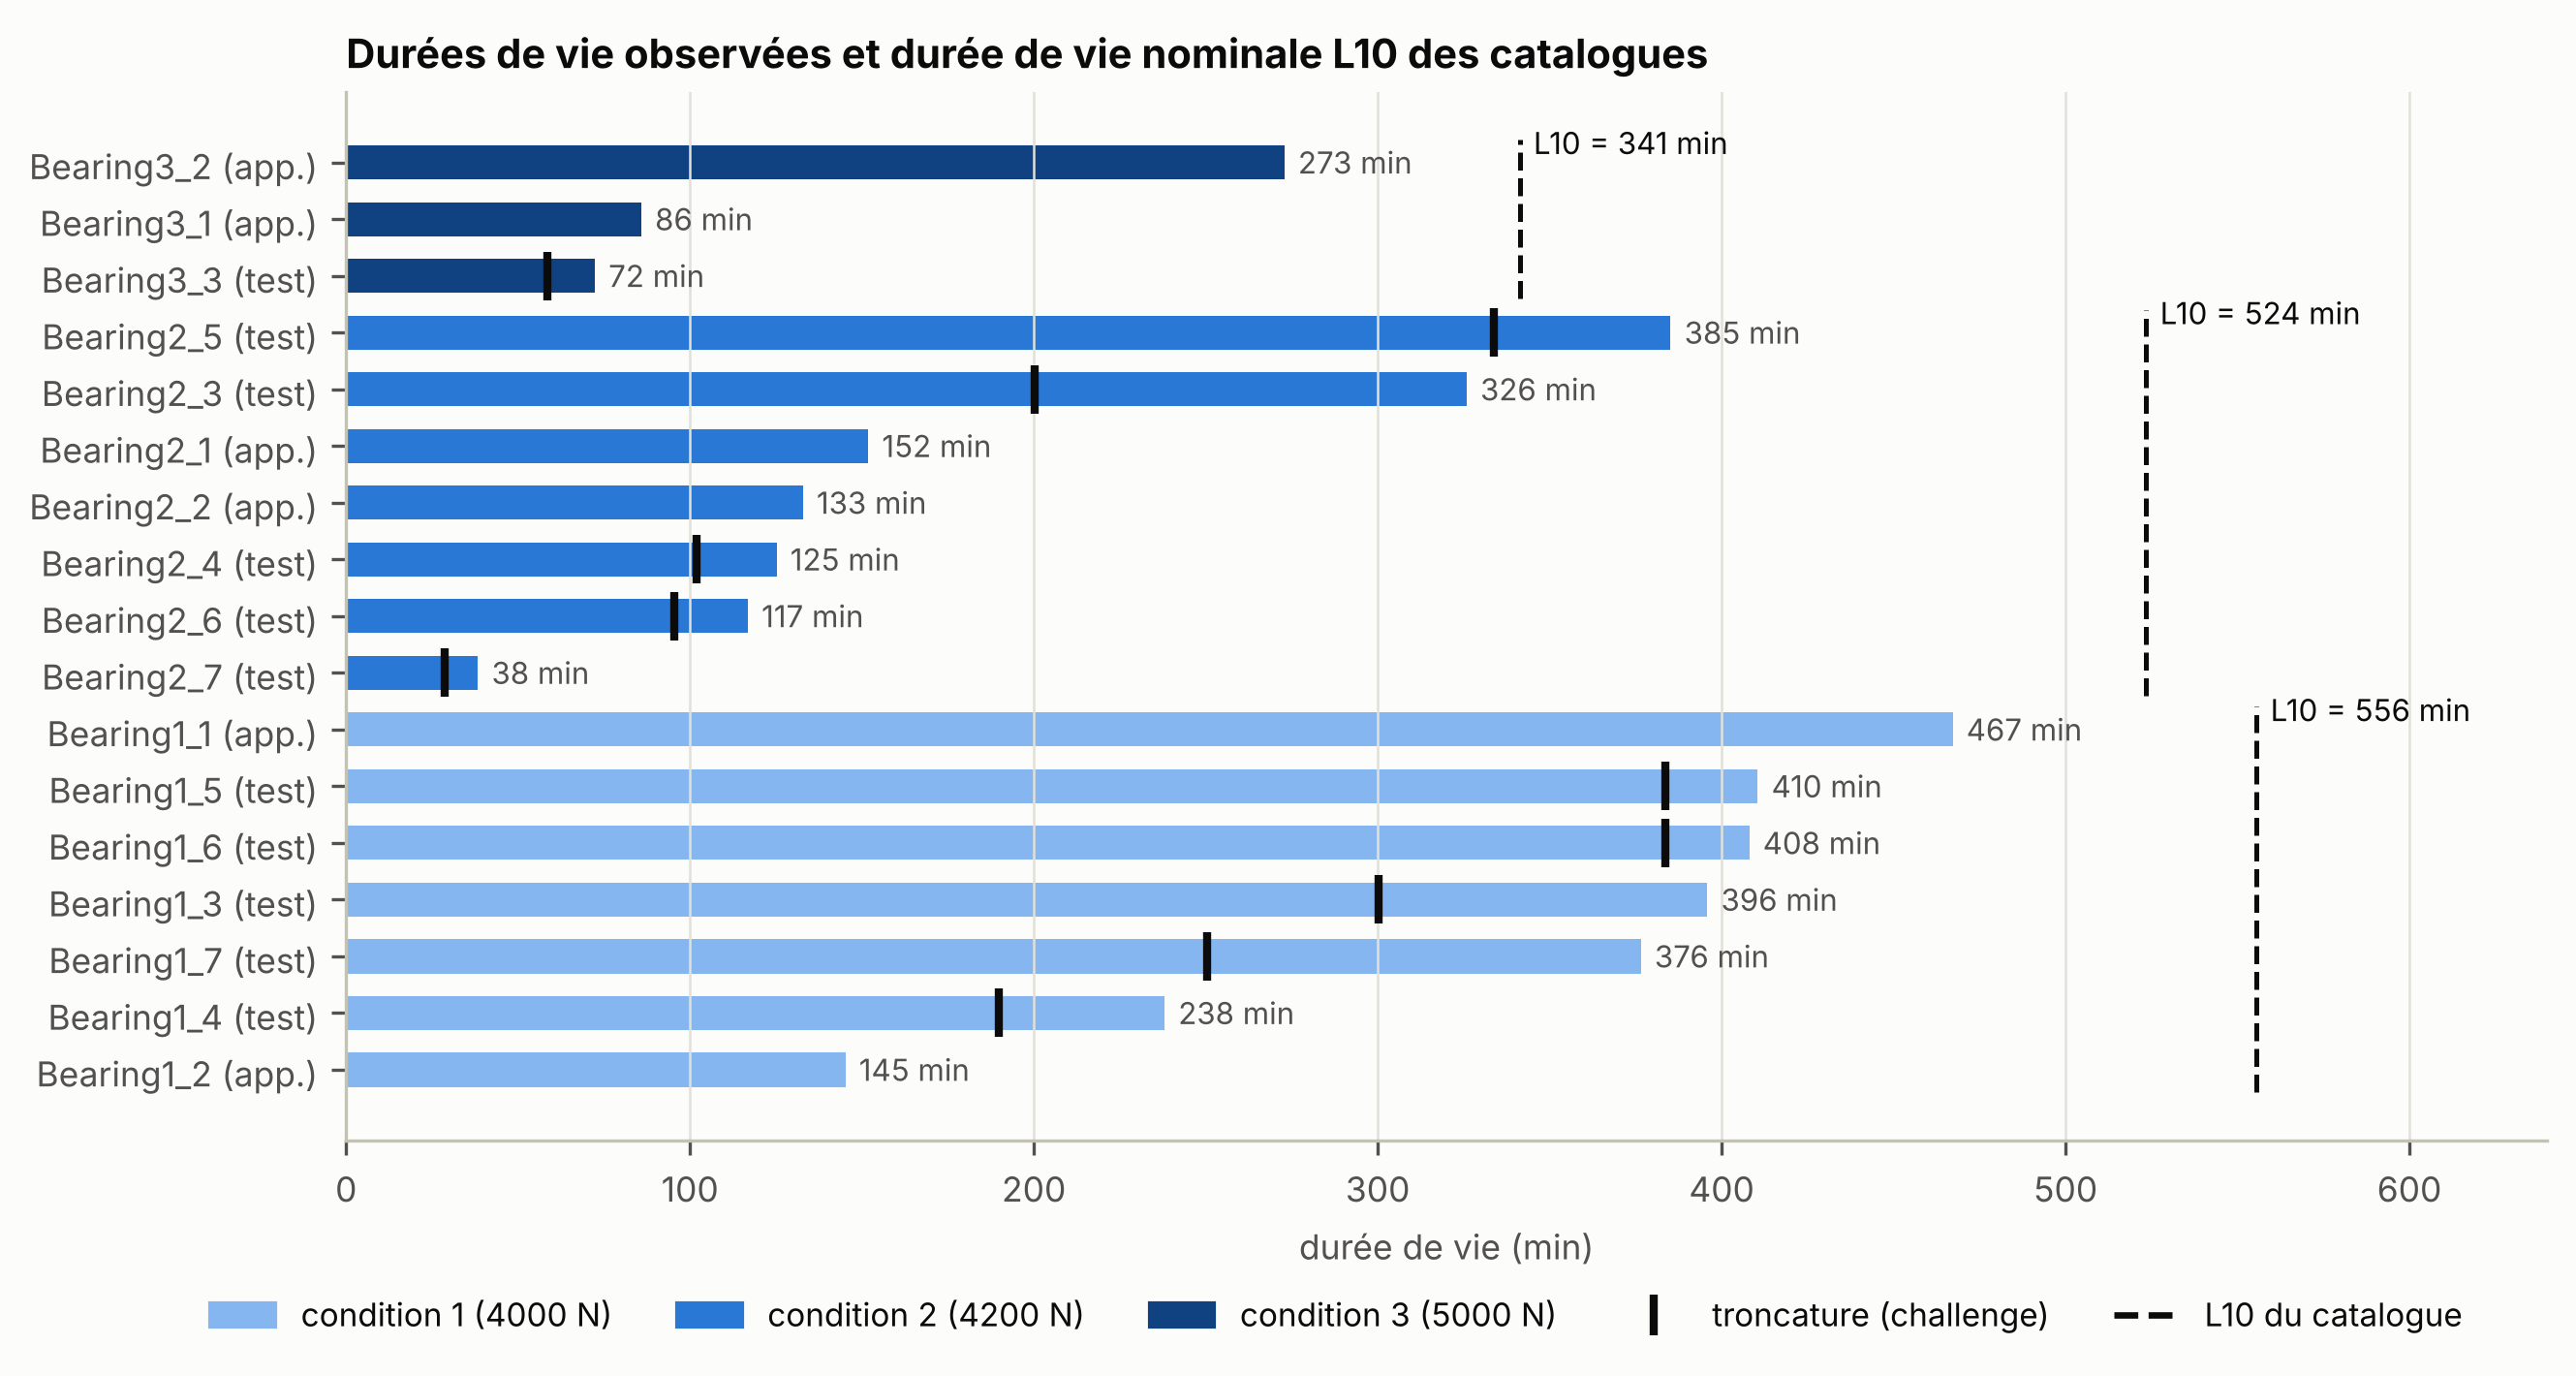
\includegraphics[width=0.8\linewidth]{figures/fig03_durees_de_vie.png}
\caption[Durées de vie des 17 roulements]{Durées de vie des 17 roulements, instants de troncature du challenge et durée L10 des catalogues.}
\label{fig:durees}
\end{figure}

\chapconclusion
Le projet suit la chaîne industrielle de la norme ISO 13374 et s'appuie sur les trois familles de méthodes de la littérature. Les données sont réelles, peu nombreuses (17 roulements) et très dispersées : il faudra être prudent dans les conclusions.

\chapter{Méthodologie de A à Z}

\chapintro
Ce chapitre décrit toute la chaîne de traitement, du fichier de vibration à la décision de maintenance. Pour chaque étape, nous expliquons la méthode simplement, puis pourquoi nous l'avons choisie.

\section{Vue d'ensemble de la démarche}

La figure~\ref{fig:pipeline} résume la démarche, et le tableau~\ref{tab:sprints} indique ce que chaque sprint a produit. Les 6 roulements d'apprentissage servent à construire et régler tout ce qui doit l'être ; les 11 roulements de test ne servent qu'à juger.

\begin{figure}[H]
\centering
\definecolor{s1}{RGB}{23,86,110}\definecolor{s2}{RGB}{31,94,67}\definecolor{s3}{RGB}{138,79,7}\definecolor{s4}{RGB}{79,51,117}
\begin{tikzpicture}[font=\small,
  bloc/.style={draw=#1,fill=#1!10,rounded corners=4pt,line width=0.9pt,minimum width=2.55cm,minimum height=1.15cm,
               align=center,text width=2.45cm},
  fleche/.style={-{Stealth[length=2.2mm]},line width=0.8pt,color=black!60}]
  \node[bloc=s1] (a) {24 889 fichiers\\de vibration};
  \node[bloc=s1,right=0.55cm of a] (b) {Contrôle qualité\\et filtrage};
  \node[bloc=s1,right=0.55cm of b] (c) {Fiabilité :\\Weibull, B10, B50};
  \node[bloc=s2,right=0.55cm of c] (d) {36 features\\normalisées};
  \node[bloc=s2,below=0.75cm of d] (e) {Premier défaut\\(règle des 3 $\sigma$)};
  \node[bloc=s2,left=0.55cm of e] (f) {Indicateur\\de santé (HI)};
  \node[bloc=s3,left=0.55cm of f] (g) {7 méthodes\\de RUL};
  \node[bloc=s4,left=0.55cm of g] (h) {Évaluation,\\tests, XAI};
  \node[bloc=s4,below=0.75cm of h,text width=5.6cm,minimum width=5.7cm] (i) {Décision de maintenance\\et analyse économique};
  \draw[fleche] (a) -- (b); \draw[fleche] (b) -- (c); \draw[fleche] (c) -- (d);
  \draw[fleche] (d) -- (e); \draw[fleche] (e) -- (f); \draw[fleche] (f) -- (g); \draw[fleche] (g) -- (h);
  \draw[fleche] (h) -- (h|-i.north);
  \node[anchor=west,font=\footnotesize,text=s1] at ($(i.east)+(0.5,0.25)$) {\textbf{Sprint 1} données};
  \node[anchor=west,font=\footnotesize,text=s2] at ($(i.east)+(3.0,0.25)$) {\textbf{Sprint 2} santé};
  \node[anchor=west,font=\footnotesize,text=s3] at ($(i.east)+(0.5,-0.25)$) {\textbf{Sprint 3} modèles};
  \node[anchor=west,font=\footnotesize,text=s4] at ($(i.east)+(3.0,-0.25)$) {\textbf{Sprint 4} évaluation};
\end{tikzpicture}
\caption[La démarche complète, du signal à la décision]{La démarche complète, du signal brut à la décision (une couleur par sprint).}
\label{fig:pipeline}
\end{figure}

\begin{table}[H]
\centering\small
\begin{tabularx}{\linewidth}{lY}
\toprule
Sprint & Travail réalisé \\
\midrule
1 · Données & lecture des fichiers, contrôle qualité, filtrage, découpage par roulement, Kaplan-Meier, Weibull, B10, B50, L10 \\
2 · Santé & 36 features, normalisation multi-conditions, détection du premier défaut, sélection des features, indicateur de santé \\
3 · Modèles & B10 conditionnel, Wiener bayésien, SVR, GPR, forêt aléatoire, LSTM, CNN 1D, recherche des hyperparamètres \\
4 · Évaluation & RMSE, MAE, score PHM, bootstrap, tests statistiques, données simulées, XAI, covariables, économie \\
\bottomrule
\end{tabularx}
\caption[Travail réalisé dans chaque sprint]{Ce que chaque sprint a produit.}
\label{tab:sprints}
\end{table}

\section{Prétraitement, features et normalisation}

\textbf{Filtrage.} On enlève la dérive lente du signal, puis on applique un filtre passe-bande de Butterworth d'ordre 4 entre 10 Hz et 10 kHz, dans les deux sens pour ne pas décaler le signal. \emph{Pourquoi :} les chocs d'un défaut de roulement sont dans cette bande ; en dessous, c'est de la dérive, au-dessus on est trop près de la limite de mesure (12,8 kHz).

\textbf{Features.} Sur chaque fichier et chaque axe, on calcule 18 indicateurs (tableau~\ref{tab:features}), soit 36 en tout. Les énergies de paquets d'ondelettes découpent le spectre en 8 bandes de 1,6 kHz et suivent l'énergie de chaque bande.

\begin{table}[H]
\centering\small
\begin{tabularx}{\linewidth}{lY}
\toprule
Famille & Indicateurs (par axe) \\
\midrule
Temporels (8) & RMS, pic, crête à crête, kurtosis, asymétrie, facteurs de crête, de forme et d'impulsion \\
Fréquentiels (2) & fréquence moyenne, entropie spectrale \\
Temps-fréquence (8) & énergie des 8 sous-bandes d'une décomposition en paquets d'ondelettes (db4, niveau 3) \\
\bottomrule
\end{tabularx}
\caption[Les 18 features par axe]{Les 18 features calculées sur chaque axe.}
\label{tab:features}
\end{table}

\textbf{Normalisation multi-conditions.} Chaque feature $x$ est divisée par son niveau à l'état sain $\bar{x}_{\text{sain}}$ (moyenne des fichiers 31 à 150, après le rodage), puis on prend le logarithme :
\begin{equation}
\tilde{x}(t) = \ln\big(x(t) / \bar{x}_{\text{sain}}\big).
\end{equation}
\emph{Pourquoi :} 0 veut alors dire « comme à l'état sain », quelles que soient la charge et la vitesse ; les trois conditions deviennent comparables. On lisse ensuite par une moyenne glissante sur 1 min, qui n'utilise que le passé.

\section{Fiabilité de la population}

\textbf{Vraisemblance avec censure.} Les 6 roulements d'apprentissage sont des défaillances ($\delta_i = 1$), les 11 roulements de test sont censurés à leur âge de troncature ($\delta_i = 0$). La vraisemblance d'une loi de densité $f$ et de fiabilité $R$ s'écrit :
\begin{equation}
L(\theta) = \prod_{i=1}^{17} f(t_i)^{\delta_i}\, R(t_i)^{1-\delta_i}.
\end{equation}
Un roulement censuré compte par $R(t_i)$ : « il a tenu au moins jusqu'à $t_i$ ». On cherche les paramètres $\theta$ qui rendent les données les plus probables (maximum de vraisemblance, MV). Nous comparons quatre lois (exponentielle, Weibull, log-normale, log-logistique) avec l'AIC $= 2k - 2\ln L$ \cite{akaike1974}, et nous testons $\beta = 1$ par le test du rapport de vraisemblance.

\textbf{Loi de Weibull et indicateurs.} Avec $R(t) = \exp\!\big(-(t/\eta)^{\beta}\big)$ \cite{benhmida2022} :
\begin{equation}
\text{MTTF} = \eta\,\Gamma(1 + 1/\beta), \qquad B_p = \eta\,\big(-\ln(1-p)\big)^{1/\beta},
\end{equation}
avec $p = 0{,}10$ pour le B10 et $p = 0{,}50$ pour le B50. Leurs intervalles de confiance sont obtenus par bootstrap \cite{efron1979} : on refait l'ajustement 1 000 fois en tirant les 17 roulements au hasard. La durée L10 des catalogues vaut $(C/P)^3$ millions de tours \cite{iso281}, avec $C = 4\,000$ N.

\textbf{B10 conditionnel.} Pour un roulement encore sain d'âge $a$, c'est la durée $x$ qu'il tiendra encore avec 90 \% de chances : $R(a + x)/R(a) = 0{,}9$. C'est notre prédiction tant qu'aucun défaut n'est détecté.

\textbf{Covariables.} Une covariable est une variable extérieure qui peut changer la durée de vie, ici la charge ou la vitesse. Le modèle de Weibull à temps accéléré (AFT) \cite{kalbfleisch2002} écrit $\ln \eta = a_0 + a_1\,z$ : chaque unité de la covariable $z$ multiplie la durée de vie par $e^{a_1}$.

\section{Premier défaut et indicateur de santé}

\textbf{Règle des 3 $\sigma$.} Pour chaque axe, le seuil vaut la moyenne plus 3 écarts-types du RMS lissé à l'état sain. On déclenche une alarme après 3 mesures de suite au-dessus du seuil, et on l'annule si le RMS repasse 5 min sous le seuil (transitoire). La règle n'utilise que le passé : elle marche en temps réel. L'instant de l'alarme confirmée est le FPT.

\textbf{Sélection des features.} Sur la phase de dégradation des roulements d'apprentissage, chaque feature reçoit trois notes entre 0 et 1 \cite{coble2009} : la \emph{monotonie} (elle évolue toujours dans le même sens), la \emph{corrélation} de Spearman avec le temps (tendance régulière) et la \emph{pronosticabilité} (tous les roulements finissent à peu près à la même valeur). Le score est la moyenne des trois notes ; les 8 meilleures features sont les entrées des modèles d'apprentissage automatique.

\textbf{Indicateur de santé.} Le HI est la moyenne des $k$ meilleures features ; on essaie $k = 1$ à 10 et on garde le meilleur score. Le seuil de défaillance $D$ est la valeur moyenne du HI à la fin de vie des roulements d'apprentissage.

\section{Les méthodes de pronostic}

\textbf{Passage d'une méthode à l'autre.} Toutes les méthodes reçoivent les mêmes données et prédisent la même chose : la RUL en minutes, à chaque instant après le FPT. On va du plus simple au plus riche (tableau~\ref{tab:methodes}) : d'abord la population (aucun capteur), puis un modèle stochastique qui suit le HI d'un seul roulement, puis l'apprentissage automatique qui combine 8 features, puis l'apprentissage profond qui lit une fenêtre de mesures successives.

\begin{table}[H]
\centering\small
\setlength{\tabcolsep}{4pt}
\begin{tabularx}{\linewidth}{lYYl}
\toprule
Méthode & Idée en une phrase & Pourquoi ce choix & Réglages testés \\
\midrule
B10 conditionnel & la population donne la durée que 90 \% des roulements de cet âge tiendront & seule réponse possible sans défaut détecté & aucun \\
Wiener bayésien & le HI monte avec une pente aléatoire ; la RUL = temps pour atteindre $D$ & explicable, donne un intervalle & aucun \\
SVR & régression à noyau qui ignore les petites erreurs & robuste avec peu de données & 24 combinaisons \\
GPR & processus gaussien, donne aussi une incertitude & lisse, bon avec peu de points & 3 combinaisons \\
Forêt aléatoire & moyenne de 300 arbres de décision & non linéaire, peu de réglages & 18 combinaisons \\
LSTM & réseau récurrent qui lit les dernières mesures & capte la dynamique & 4 combinaisons \\
CNN 1D & convolutions sur une fenêtre de mesures & rapide, motifs locaux & 4 combinaisons \\
\bottomrule
\end{tabularx}
\caption[Les sept méthodes de pronostic]{Les sept méthodes de pronostic comparées.}
\label{tab:methodes}
\end{table}

\textbf{Le processus de Wiener bayésien.} Après le FPT, le HI suit $X(t) = X(t_0) + \mu\,(t - t_0) + \sigma B(t - t_0)$, où $B$ est un mouvement brownien \cite{si2011,zhang2018}. La pente $\mu$ change d'un roulement à l'autre : on lui donne une loi \emph{a priori} $\mathcal{N}(\mu_0, s_0^2)$ apprise sur l'apprentissage, puis on la met à jour avec la montée observée du roulement suivi :
\begin{equation}
\mu_{\text{post}} = \frac{\mu_0/s_0^2 + \Delta X/\sigma^2}{1/s_0^2 + \Delta t/\sigma^2}.
\end{equation}
Au début on fait confiance à la population, puis de plus en plus au roulement lui-même. Le seuil $D$ est lui aussi incertain. En tirant 2 000 couples $(\mu, D)$, le temps de premier passage (loi inverse gaussienne) donne la RUL médiane et un intervalle de prédiction à 90 \%.

\textbf{Apprentissage automatique et profond.} Entrées : les 8 features et le temps écoulé depuis le FPT. Cible : $\ln(1 + \text{RUL})$, pour que les erreurs proches de la fin de vie comptent plus. Chaque roulement d'apprentissage donne 100 exemples, pour peser autant que les autres.

\textbf{Changement des paramètres.} Les hyperparamètres sont choisis par recherche sur grille avec une validation croisée « un roulement de côté » : on apprend sur 5 roulements d'apprentissage et on valide sur le 6\textsuperscript{e}, six fois. Le test ne sert jamais au réglage.

\section{Critères de jugement, protocoles et tests}

\textbf{Critères.} Sur toute la phase de dégradation, on calcule la RMSE et la MAE (en minutes) de chaque roulement, puis leur moyenne. Le challenge juge aussi une prédiction ponctuelle par son erreur relative et un score asymétrique :
\begin{equation}
\%Er = 100\,\frac{\text{RUL}_{\text{réelle}} - \text{RUL}_{\text{prédite}}}{\text{RUL}_{\text{réelle}}}, \qquad
A = \begin{cases} e^{-\ln(0{,}5)\,\%Er/5} & \text{si } \%Er \le 0 \text{ (trop tard)}\\ e^{+\ln(0{,}5)\,\%Er/20} & \text{si } \%Er > 0 \text{ (trop tôt)} \end{cases}
\end{equation}
Prévoir 5 \% trop tard coûte autant que prévoir 20 \% trop tôt : une panne surprise est plus grave qu'un remplacement un peu précoce. Le \emph{score PHM} est la moyenne de $A$ à 25, 50 et 75 \% de la phase de dégradation de chaque roulement ; le \emph{score challenge} prend une seule prédiction, à l'instant de troncature. Pour le Wiener, on mesure aussi la \emph{couverture} : la part des vraies RUL qui tombent dans l'intervalle à 90 \%.

\textbf{Différents types de tests.} Nous avons vérifié le travail de six façons (tableau~\ref{tab:tests}).

\begin{table}[H]
\centering\small
\begin{tabularx}{\linewidth}{lY}
\toprule
Type de test & Question posée \\
\midrule
Tests unitaires (29 tests pytest) & chaque fonction donne-t-elle la réponse connue à la main ? \\
Données simulées & la méthode retrouve-t-elle la vérité quand on la connaît ? \\
Validation croisée « un roulement de côté » & les réglages sont-ils choisis sans regarder le test ? \\
Test indépendant (11 roulements) & le modèle marche-t-il sur des roulements jamais vus ? \\
Tests statistiques & les écarts entre méthodes sont-ils réels (Wilcoxon \cite{wilcoxon1945}, Friedman \cite{friedman1937}) ? \\
Bootstrap & quelle est l'incertitude des indicateurs et des scores ? \\
\bottomrule
\end{tabularx}
\caption[Les six types de tests]{Les six façons de tester le travail.}
\label{tab:tests}
\end{table}

\section{Modèle économique}

On compare plusieurs stratégies en rejouant la vie des 11 roulements de test. Un remplacement planifié coûte $C_p = 1$ unité (u), une panne coûte $C_c = 5$ u (urgence, arrêt, dégâts) et une fausse alarme coûte une inspection à 0,1 u. Pour la stratégie préventive, le coût moyen par heure d'un remplacement à l'âge $T$ est \cite{barlow1965} :
\begin{equation}
C(T) = \frac{C_p\,R(T) + C_c\,\big(1 - R(T)\big)}{\int_0^T R(u)\,du},
\end{equation}
et l'âge optimal $T^*$ minimise $C(T)$. Pour les stratégies prédictives, on déclenche le remplacement dès que la RUL prédite passe sous un seuil $s = 10$ min ; il a lieu après un délai d'intervention de 2 min. S'il arrive avant la panne, on paie $C_p$ ; sinon, on paie $C_c$.

\chapconclusion
La démarche couvre les six blocs de la surveillance industrielle, avec une règle simple : tout ce qui se règle l'est sur l'apprentissage, tout ce qui se juge l'est sur le test.

\chapter{Résultats, benchmark et analyse}

\chapintro
Ce chapitre présente les résultats dans l'ordre de la démarche : la fiabilité de la population, la santé des roulements, puis la comparaison des sept méthodes de pronostic. Il se termine par la validation sur données simulées, l'explicabilité et le tableau de bord.

\section{Fiabilité de la population}

\subsection{Choix de la loi par la vraisemblance}
Le tableau~\ref{tab:lois} compare les quatre lois ajustées par maximum de vraisemblance, en tenant compte des 11 roulements censurés. Les trois lois à deux paramètres sont presque équivalentes (écart d'AIC inférieur à 2) ; la log-normale est à peine meilleure. Nous gardons la \textbf{loi de Weibull}, la référence en fiabilité, parce que son paramètre $\beta$ s'interprète directement (usure ou non) et donne le B10 par une formule simple.

\begin{table}[H]
\centering\small
\begin{tabular}{lccc}
\toprule
Loi & Paramètres & Log-vraisemblance & AIC \\
\midrule
Exponentielle & 1 & $-44{,}35$ & 90,70 \\
\textbf{Weibull} & 2 & $-42{,}98$ & 89,95 \\
Log-normale & 2 & $-42{,}65$ & 89,31 \\
Log-logistique & 2 & $-42{,}98$ & 89,96 \\
\bottomrule
\end{tabular}
\caption[Comparaison des lois par la vraisemblance]{Comparaison des lois de durée de vie (maximum de vraisemblance avec censure).}
\label{tab:lois}
\end{table}

La figure~\ref{fig:vraisemblance} montre les lois face à l'estimateur de Kaplan-Meier, et la surface de vraisemblance de Weibull : le maximum est atteint en $\beta = 1{,}85$ et $\eta = 422$ min, mais la région de confiance à 95 \% est très large. Le test du rapport de vraisemblance ($\beta = 1$ contre $\beta$ libre) donne $p = 0{,}097$ : avec seulement 6 défaillances, on ne peut pas \emph{prouver} l'usure au seuil de 5 \%. L'intervalle bootstrap de $\beta$, de 1,31 à 3,37, reste pourtant au-dessus de 1 : l'usure est probable.

\begin{figure}[H]
\centering
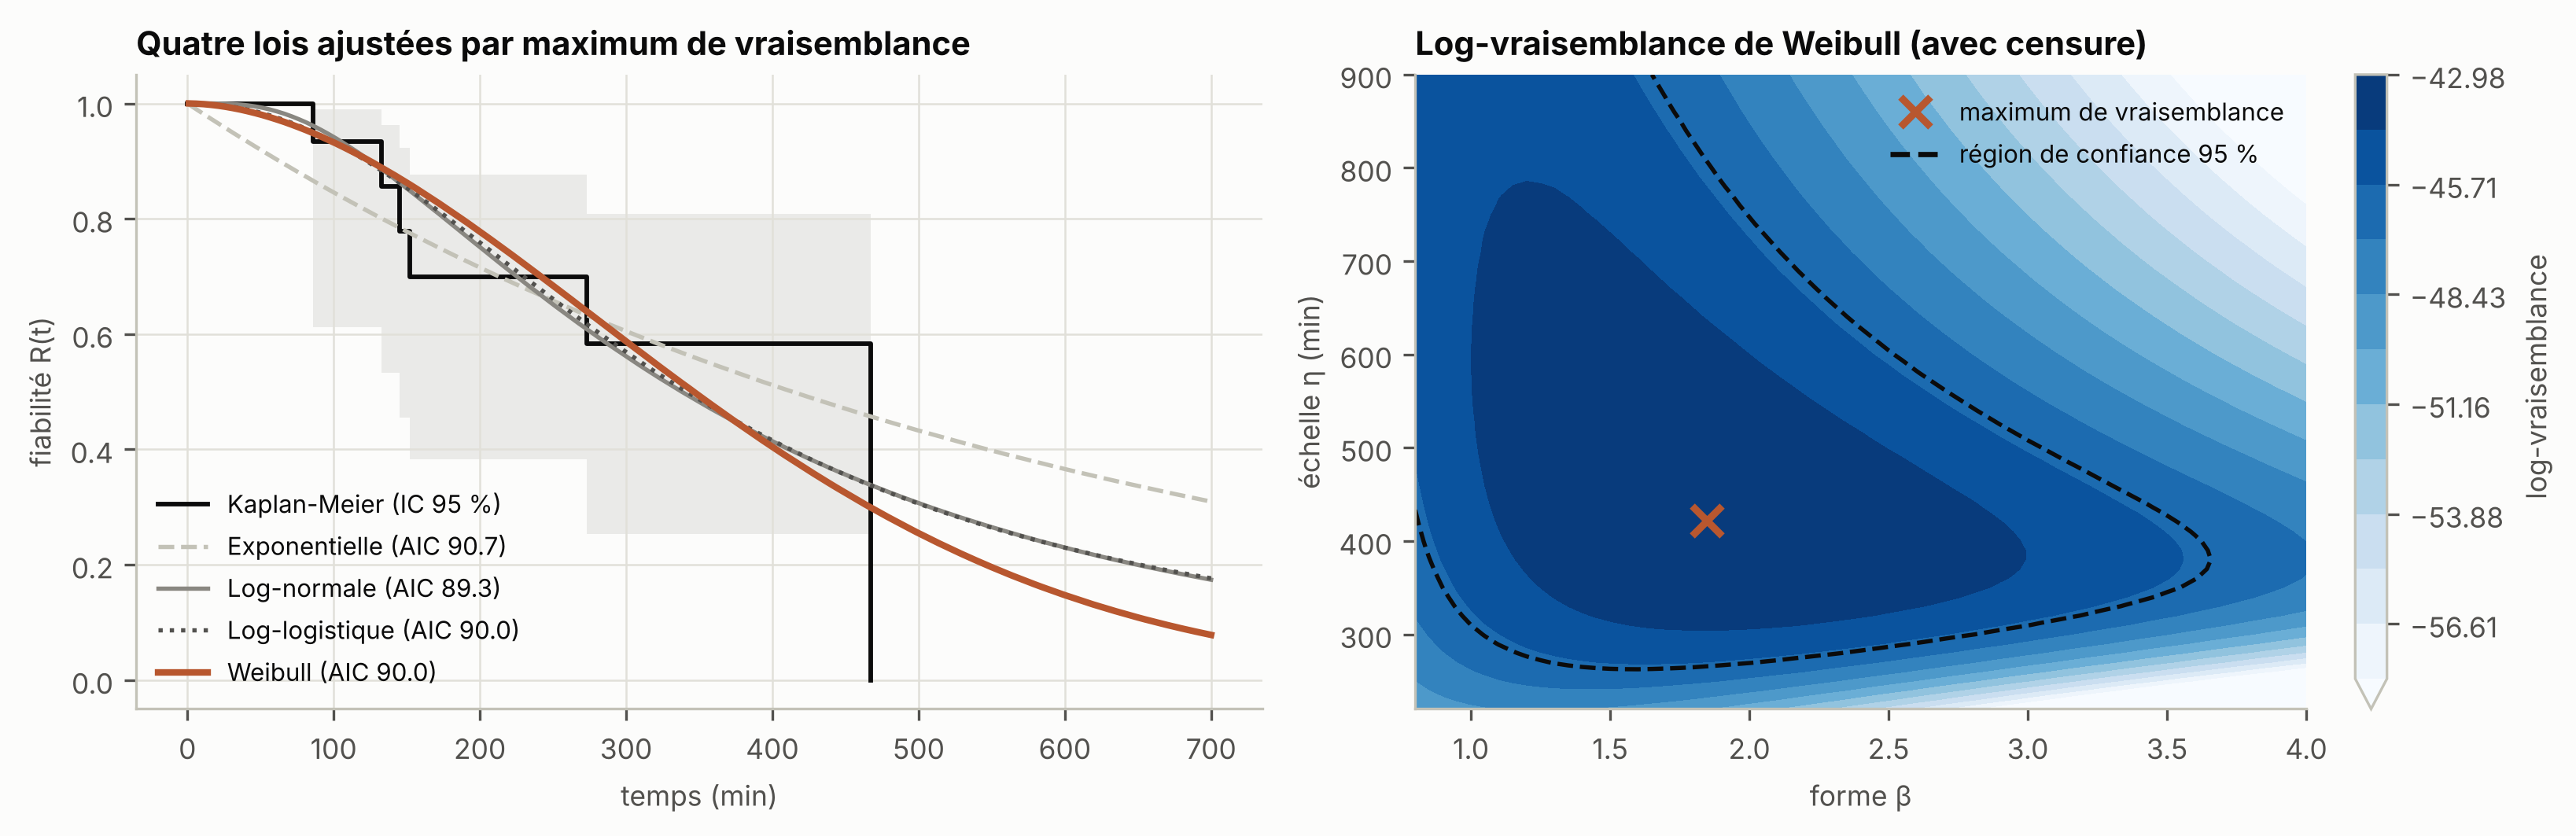
\includegraphics[width=\linewidth]{figures/fig18_vraisemblance.png}
\caption[Lois ajustées et surface de vraisemblance]{À gauche : quatre lois ajustées face à Kaplan-Meier. À droite : log-vraisemblance de Weibull, son maximum et la région de confiance à 95 \%.}
\label{fig:vraisemblance}
\end{figure}

\subsection{Indicateurs de fiabilité : B10, B50 et MTTF}
Le tableau~\ref{tab:fiabilite} donne les indicateurs, avec leurs intervalles de confiance à 95 \% obtenus par bootstrap. Un roulement sur dix casse avant 125 min et la moitié avant 346 min. Les intervalles sont larges : c'est le prix de 17 roulements seulement. La figure~\ref{fig:fiabilite} montre que le taux de défaillance augmente avec l'âge, et que le B10 conditionnel d'un roulement sain diminue quand il vieillit.

\begin{table}[H]
\centering\small
\begin{tabular}{lcc}
\toprule
Indicateur & Valeur & IC 95 \% (bootstrap) \\
\midrule
Forme $\beta$ & 1,85 & [1,31 ; 3,37] \\
Échelle $\eta$ & 422 min & [261 ; 732] min \\
MTTF & 375 min & [232 ; 666] min \\
B10 & 125 min & [78 ; 234] min \\
B50 (médiane) & 346 min & [219 ; 573] min \\
L10 des catalogues (conditions 1 / 2 / 3) & 556 / 524 / 341 min & — \\
\bottomrule
\end{tabular}
\caption[Indicateurs de fiabilité]{Indicateurs de fiabilité de la population (loi de Weibull).}
\label{tab:fiabilite}
\end{table}

\begin{figure}[H]
\centering
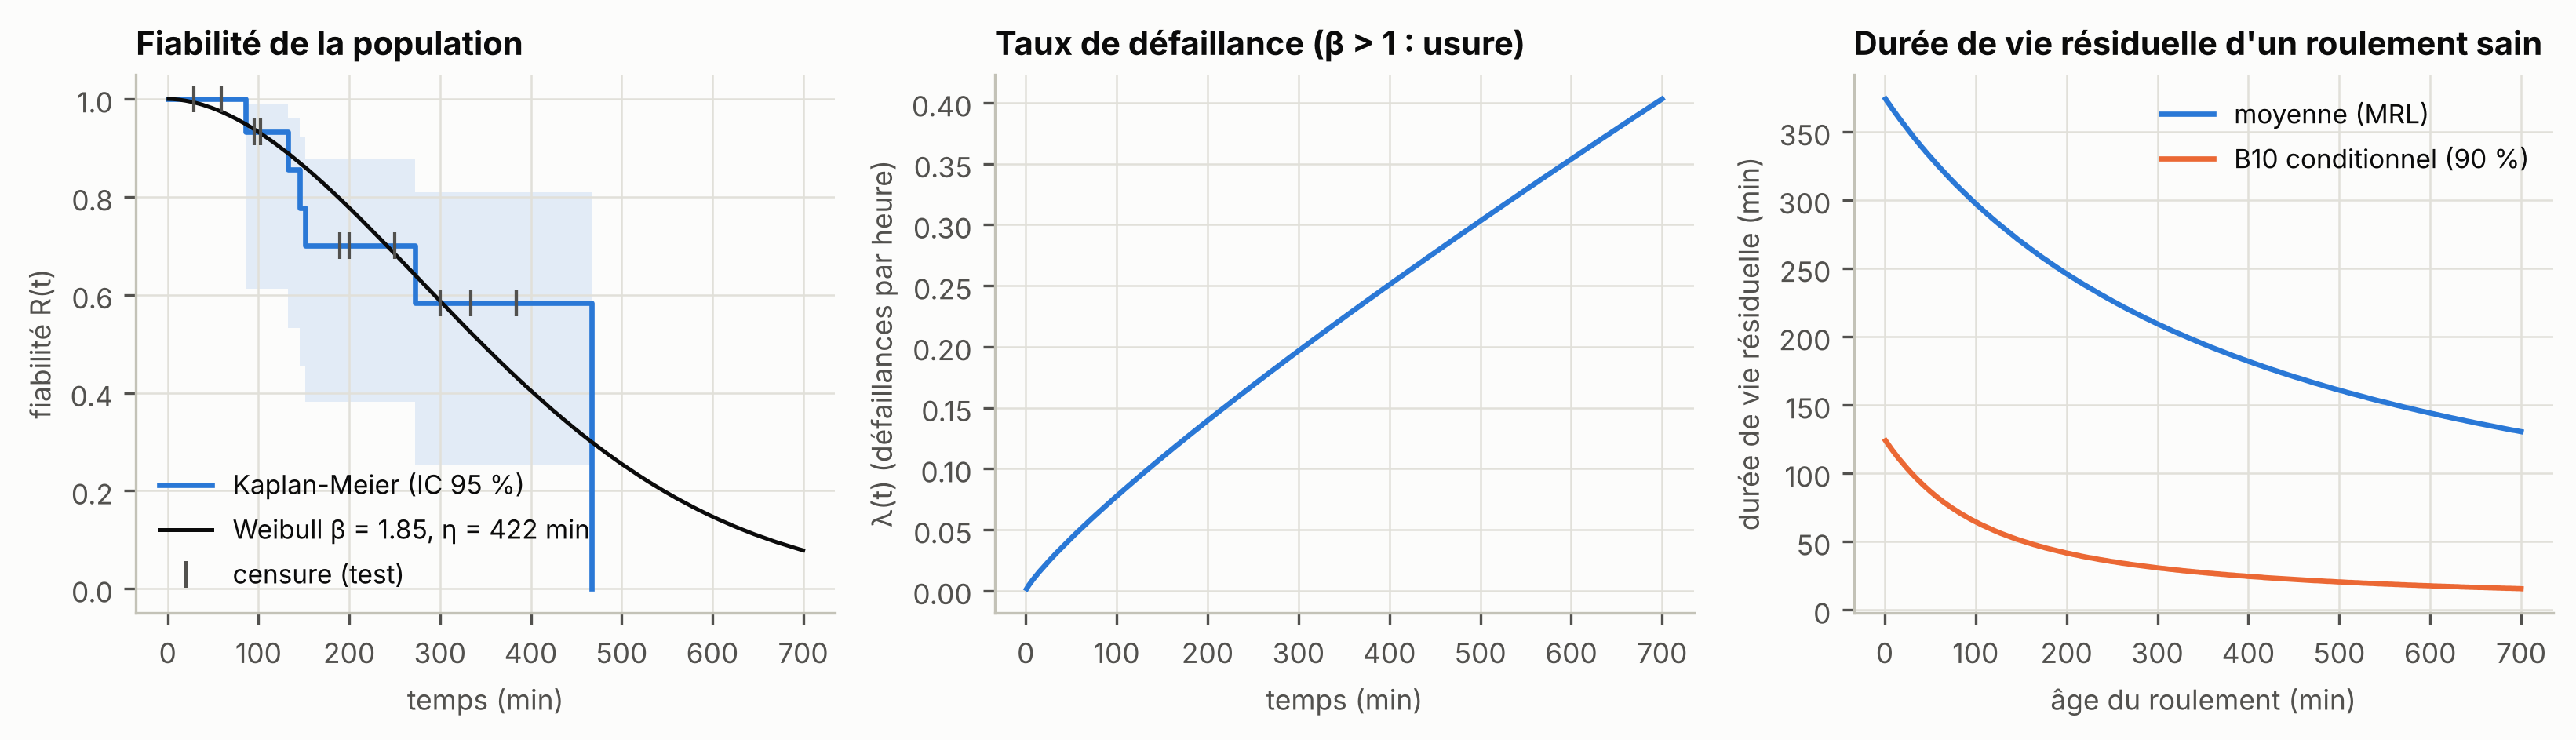
\includegraphics[width=\linewidth]{figures/fig04_fiabilite.png}
\caption[Fiabilité, taux de défaillance et B10 conditionnel]{Fiabilité de la population : Kaplan-Meier et Weibull, taux de défaillance, durée de vie résiduelle d'un roulement sain.}
\label{fig:fiabilite}
\end{figure}

La plupart des roulements cassent bien avant leur L10 (figure~\ref{fig:durees}) : la formule des catalogues ne s'applique pas à ces essais accélérés, ce que notent aussi les organisateurs du challenge \cite{phm2012challenge}.

\subsection{Ajout de covariables}
La figure~\ref{fig:covariables} ajoute la charge comme covariable (modèle AFT). \textbf{Un kilonewton de plus multiplie la durée de vie par 0,40} ($p = 0{,}042$), et l'AIC baisse de 90,0 à 88,3 : la covariable améliore le modèle. Le B10 passe de 175 min sous la condition 1 à 69 min sous la condition 3. La vitesse ($p = 0{,}033$) et la durée L10 ($p = 0{,}049$) donnent des conclusions semblables. Attention : la vitesse baisse quand la charge monte, et il n'y a que trois conditions ; les deux effets sont donc mélangés.

\begin{figure}[H]
\centering
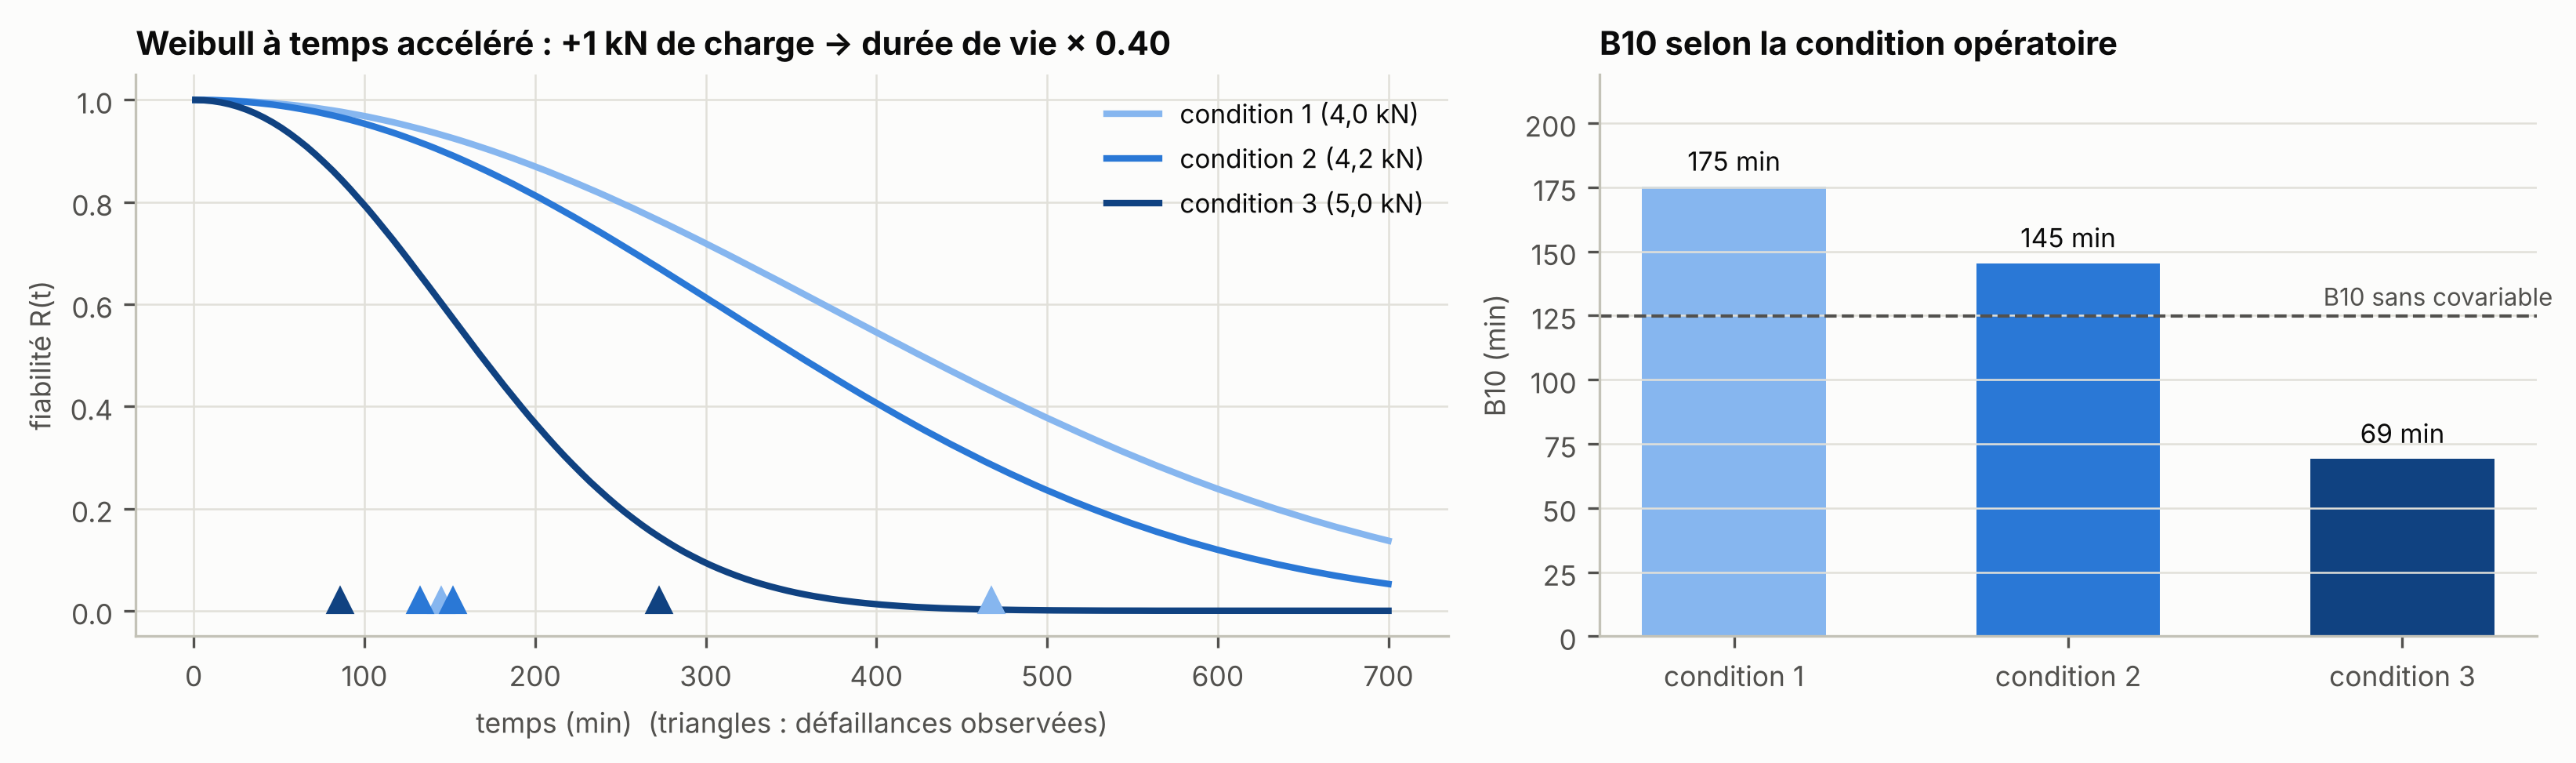
\includegraphics[width=\linewidth]{figures/fig19_covariables.png}
\caption[Effet de la charge (covariable)]{Effet de la charge sur la fiabilité (Weibull à temps accéléré) et B10 par condition.}
\label{fig:covariables}
\end{figure}

\section{Premier défaut et indicateur de santé}

La figure~\ref{fig:fpt} montre la règle des 3 $\sigma$ sur deux roulements : les alarmes passagères sont annulées, et seule l'alarme qui dure est retenue. Sur les 17 roulements, l'alarme arrive en médiane \textbf{7,8 min avant la panne} ; 14 fausses alarmes ont été annulées. À l'instant de troncature du challenge, \textbf{8 roulements de test sur 11 ne montrent encore aucun défaut} : seuls Bearing1\_3, Bearing1\_4 et Bearing3\_3 sont dégradés.

\begin{figure}[H]
\centering
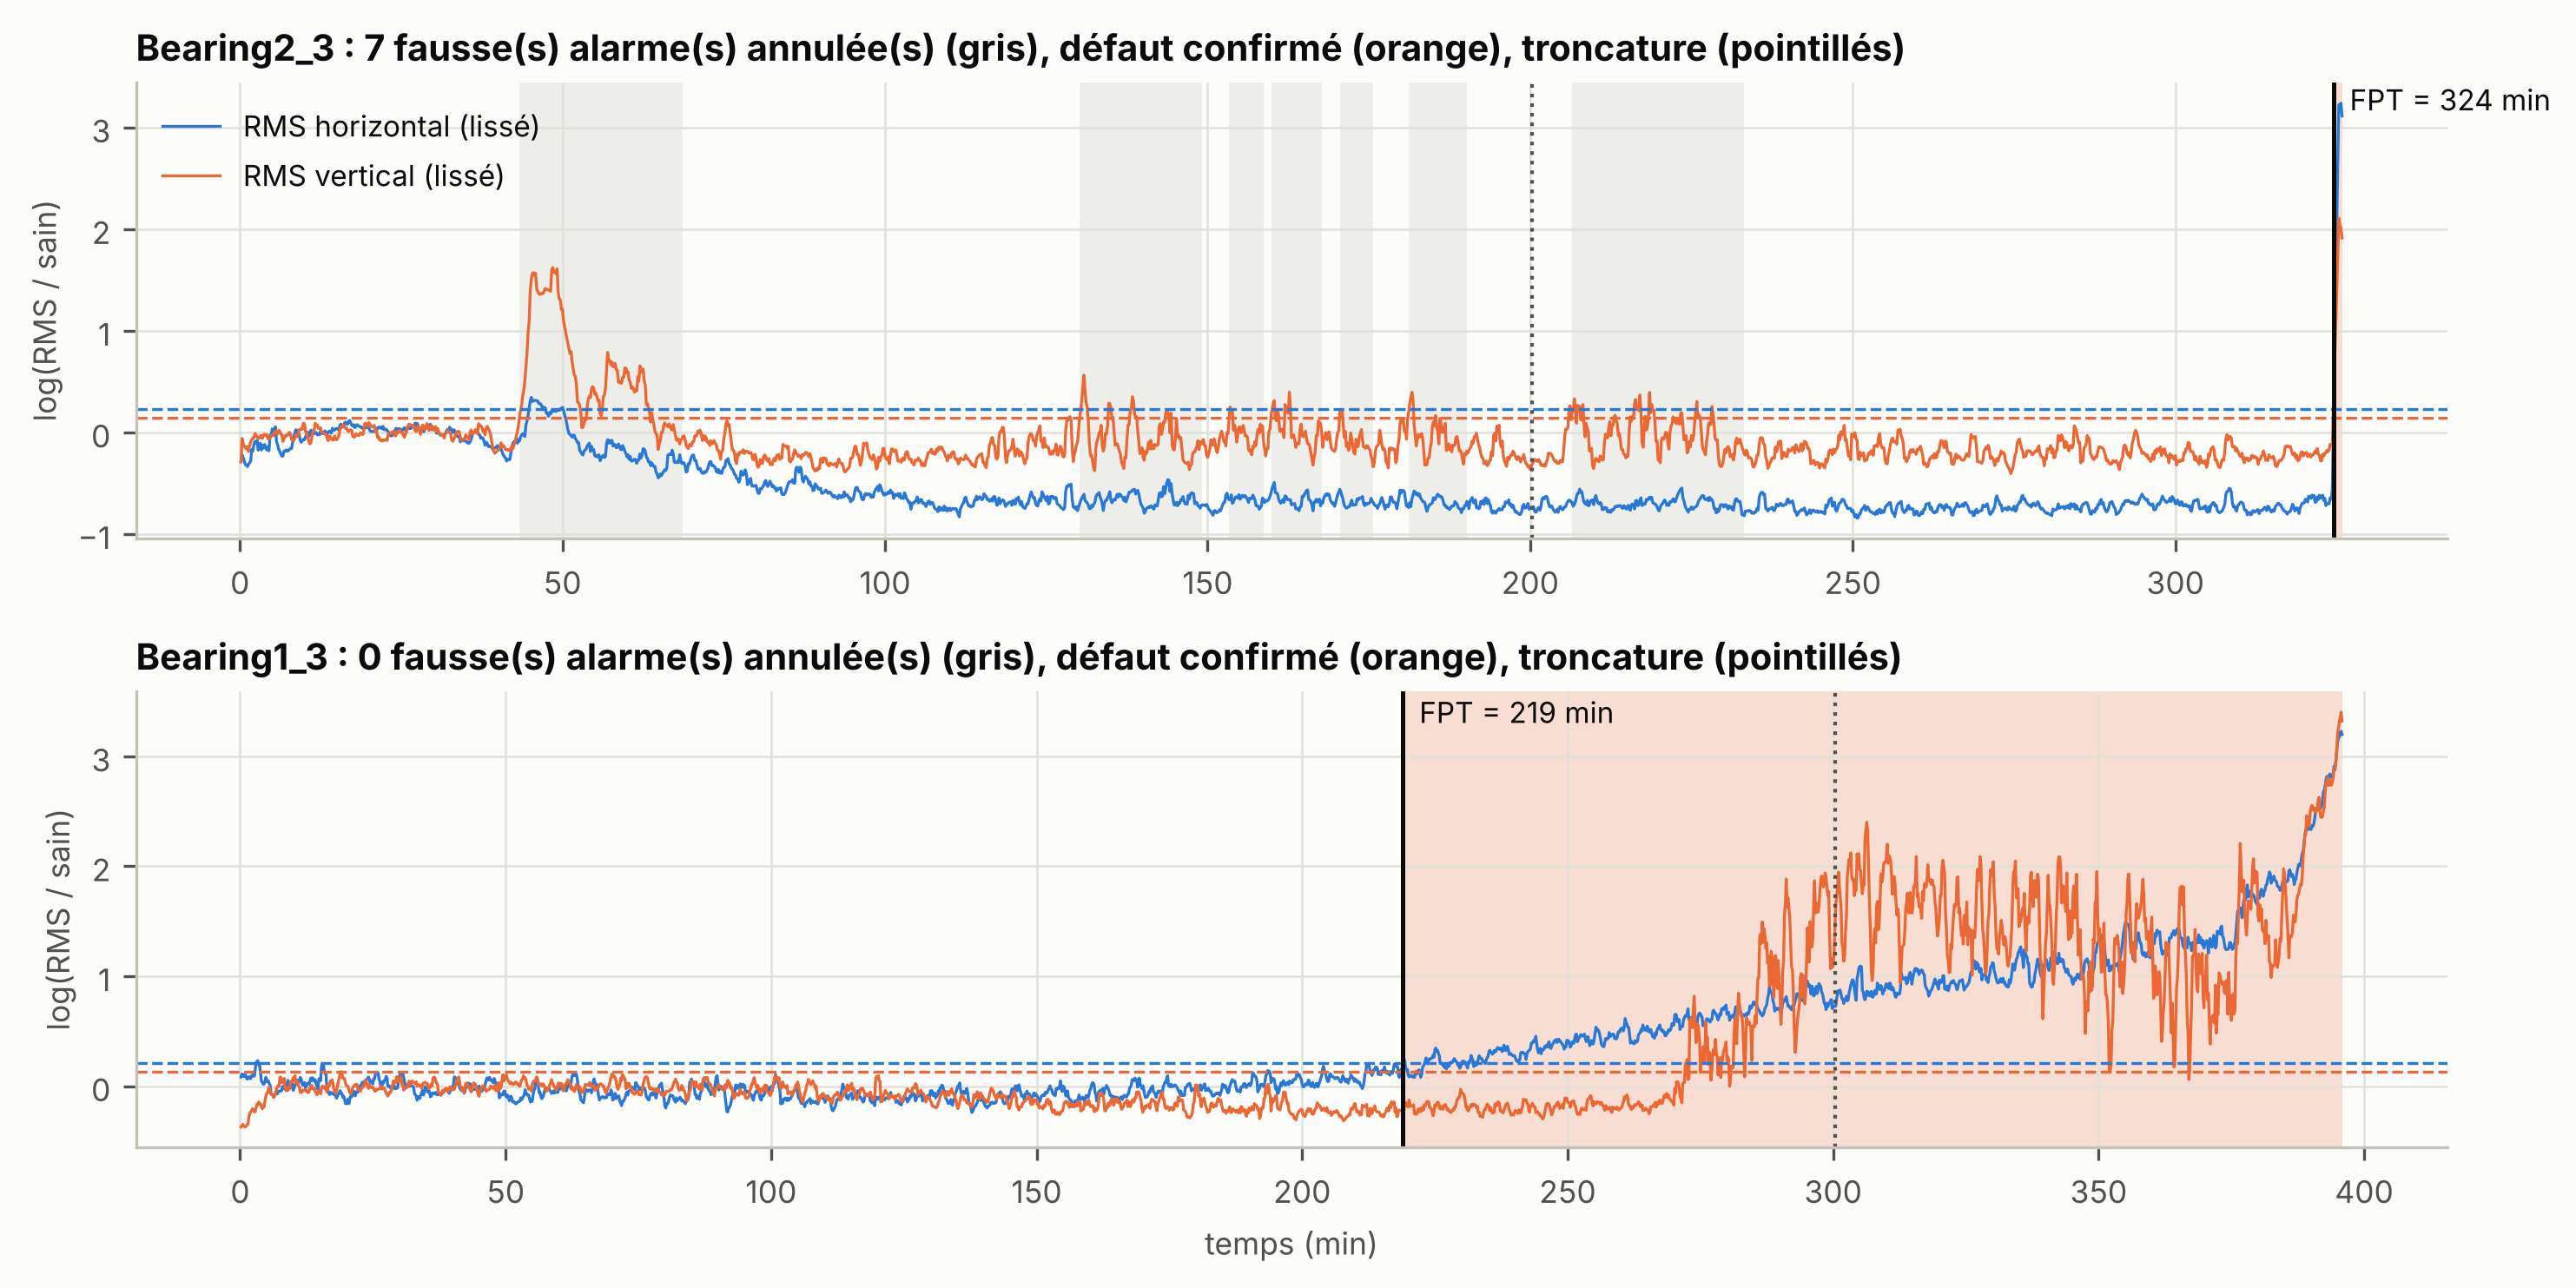
\includegraphics[width=0.86\linewidth]{figures/fig06_detection_fpt.png}
\caption[Détection du premier défaut (règle des 3 $\sigma$)]{Détection du premier défaut par la règle des 3 $\sigma$ (zones grises : fausses alarmes annulées).}
\label{fig:fpt}
\end{figure}

\textbf{Changement du seuil.} Le tableau~\ref{tab:sensibilite} montre l'effet du seuil de détection. Un seuil bas donne plus de fausses alarmes ; un seuil haut prévient plus tard. Le seuil de 3 $\sigma$ est un bon compromis.

\begin{table}[H]
\centering\small
\begin{tabular}{ccccc}
\toprule
Seuil & Fausses alarmes & Délai d'alerte médian & Délai d'alerte moyen & Tests dégradés \\
\midrule
2 $\sigma$ & 25 & 8,0 min & 43,3 min & 3 \\
\textbf{3 $\sigma$} & 14 & 7,8 min & 39,5 min & 3 \\
4 $\sigma$ & 18 & 6,8 min & 30,6 min & 3 \\
5 $\sigma$ & 11 & 6,8 min & 27,0 min & 3 \\
\bottomrule
\end{tabular}
\caption[Sensibilité au seuil de détection]{Sensibilité de la détection au seuil (17 roulements ; dernière colonne : roulements de test déjà dégradés à la troncature).}
\label{tab:sensibilite}
\end{table}

\textbf{Indicateur de santé.} Les 8 meilleures features sont toutes des énergies de bandes d'ondelettes. Le meilleur HI est une seule feature, l'énergie de la bande 6,4–8,0 kHz de l'axe vertical : score 0,644, contre 0,599 pour la moyenne des 8 meilleures. Moyenner rend la fin de vie plus régulière, mais casse la tendance. Le seuil de défaillance vaut $D = 3{,}34 \pm 0{,}63$.

\section{Pronostic de la RUL : benchmark des méthodes}

\subsection{Résultats sur la phase de dégradation}
Le tableau~\ref{tab:resultats} résume les résultats sur les 11 roulements de test. Après le premier défaut, \textbf{toutes les méthodes fondées sur les capteurs battent la fiabilité seule} : RMSE de 16 à 23 min contre 44 min. Le \textbf{processus de Wiener} est le plus précis (RMSE 16,4 min) et le meilleur selon le protocole officiel (score 0,194). Le \textbf{LSTM} a le meilleur score PHM (0,084) : il prédit moins souvent trop tard.

\begin{table}[H]
\centering\small
\begin{tabular}{lccccr}
\toprule
Méthode & RMSE (min) & MAE (min) & Score PHM & Score challenge & Apprentissage \\
\midrule
Fiabilité (B10) & 44,4 & 42,8 & 0,044 & 0,170 & — \\
\textbf{Wiener} & \textbf{16,4} & \textbf{13,0} & 0,059 & \textbf{0,194} & < 0,1 s \\
SVR & 20,0 & 17,1 & 0,059 & 0,175 & 6,5 s \\
GPR & 18,3 & 15,3 & 0,064 & 0,171 & 6,6 s \\
Forêt aléatoire & 23,0 & 18,1 & 0,059 & 0,169 & 14,3 s \\
\textbf{LSTM} & 18,7 & 15,2 & \textbf{0,084} & 0,187 & 200 s \\
CNN 1D & 17,9 & 15,3 & 0,063 & 0,169 & 142 s \\
\bottomrule
\end{tabular}
\caption[Résultats des sept méthodes]{Résultats des sept méthodes sur les 11 roulements de test.}
\label{tab:resultats}
\end{table}

La figure~\ref{fig:trajectoires} montre les RUL prédites au fil du temps sur quatre roulements de test, et la figure~\ref{fig:comparaison} les métriques avec leurs intervalles de confiance.

\begin{figure}[H]
\centering
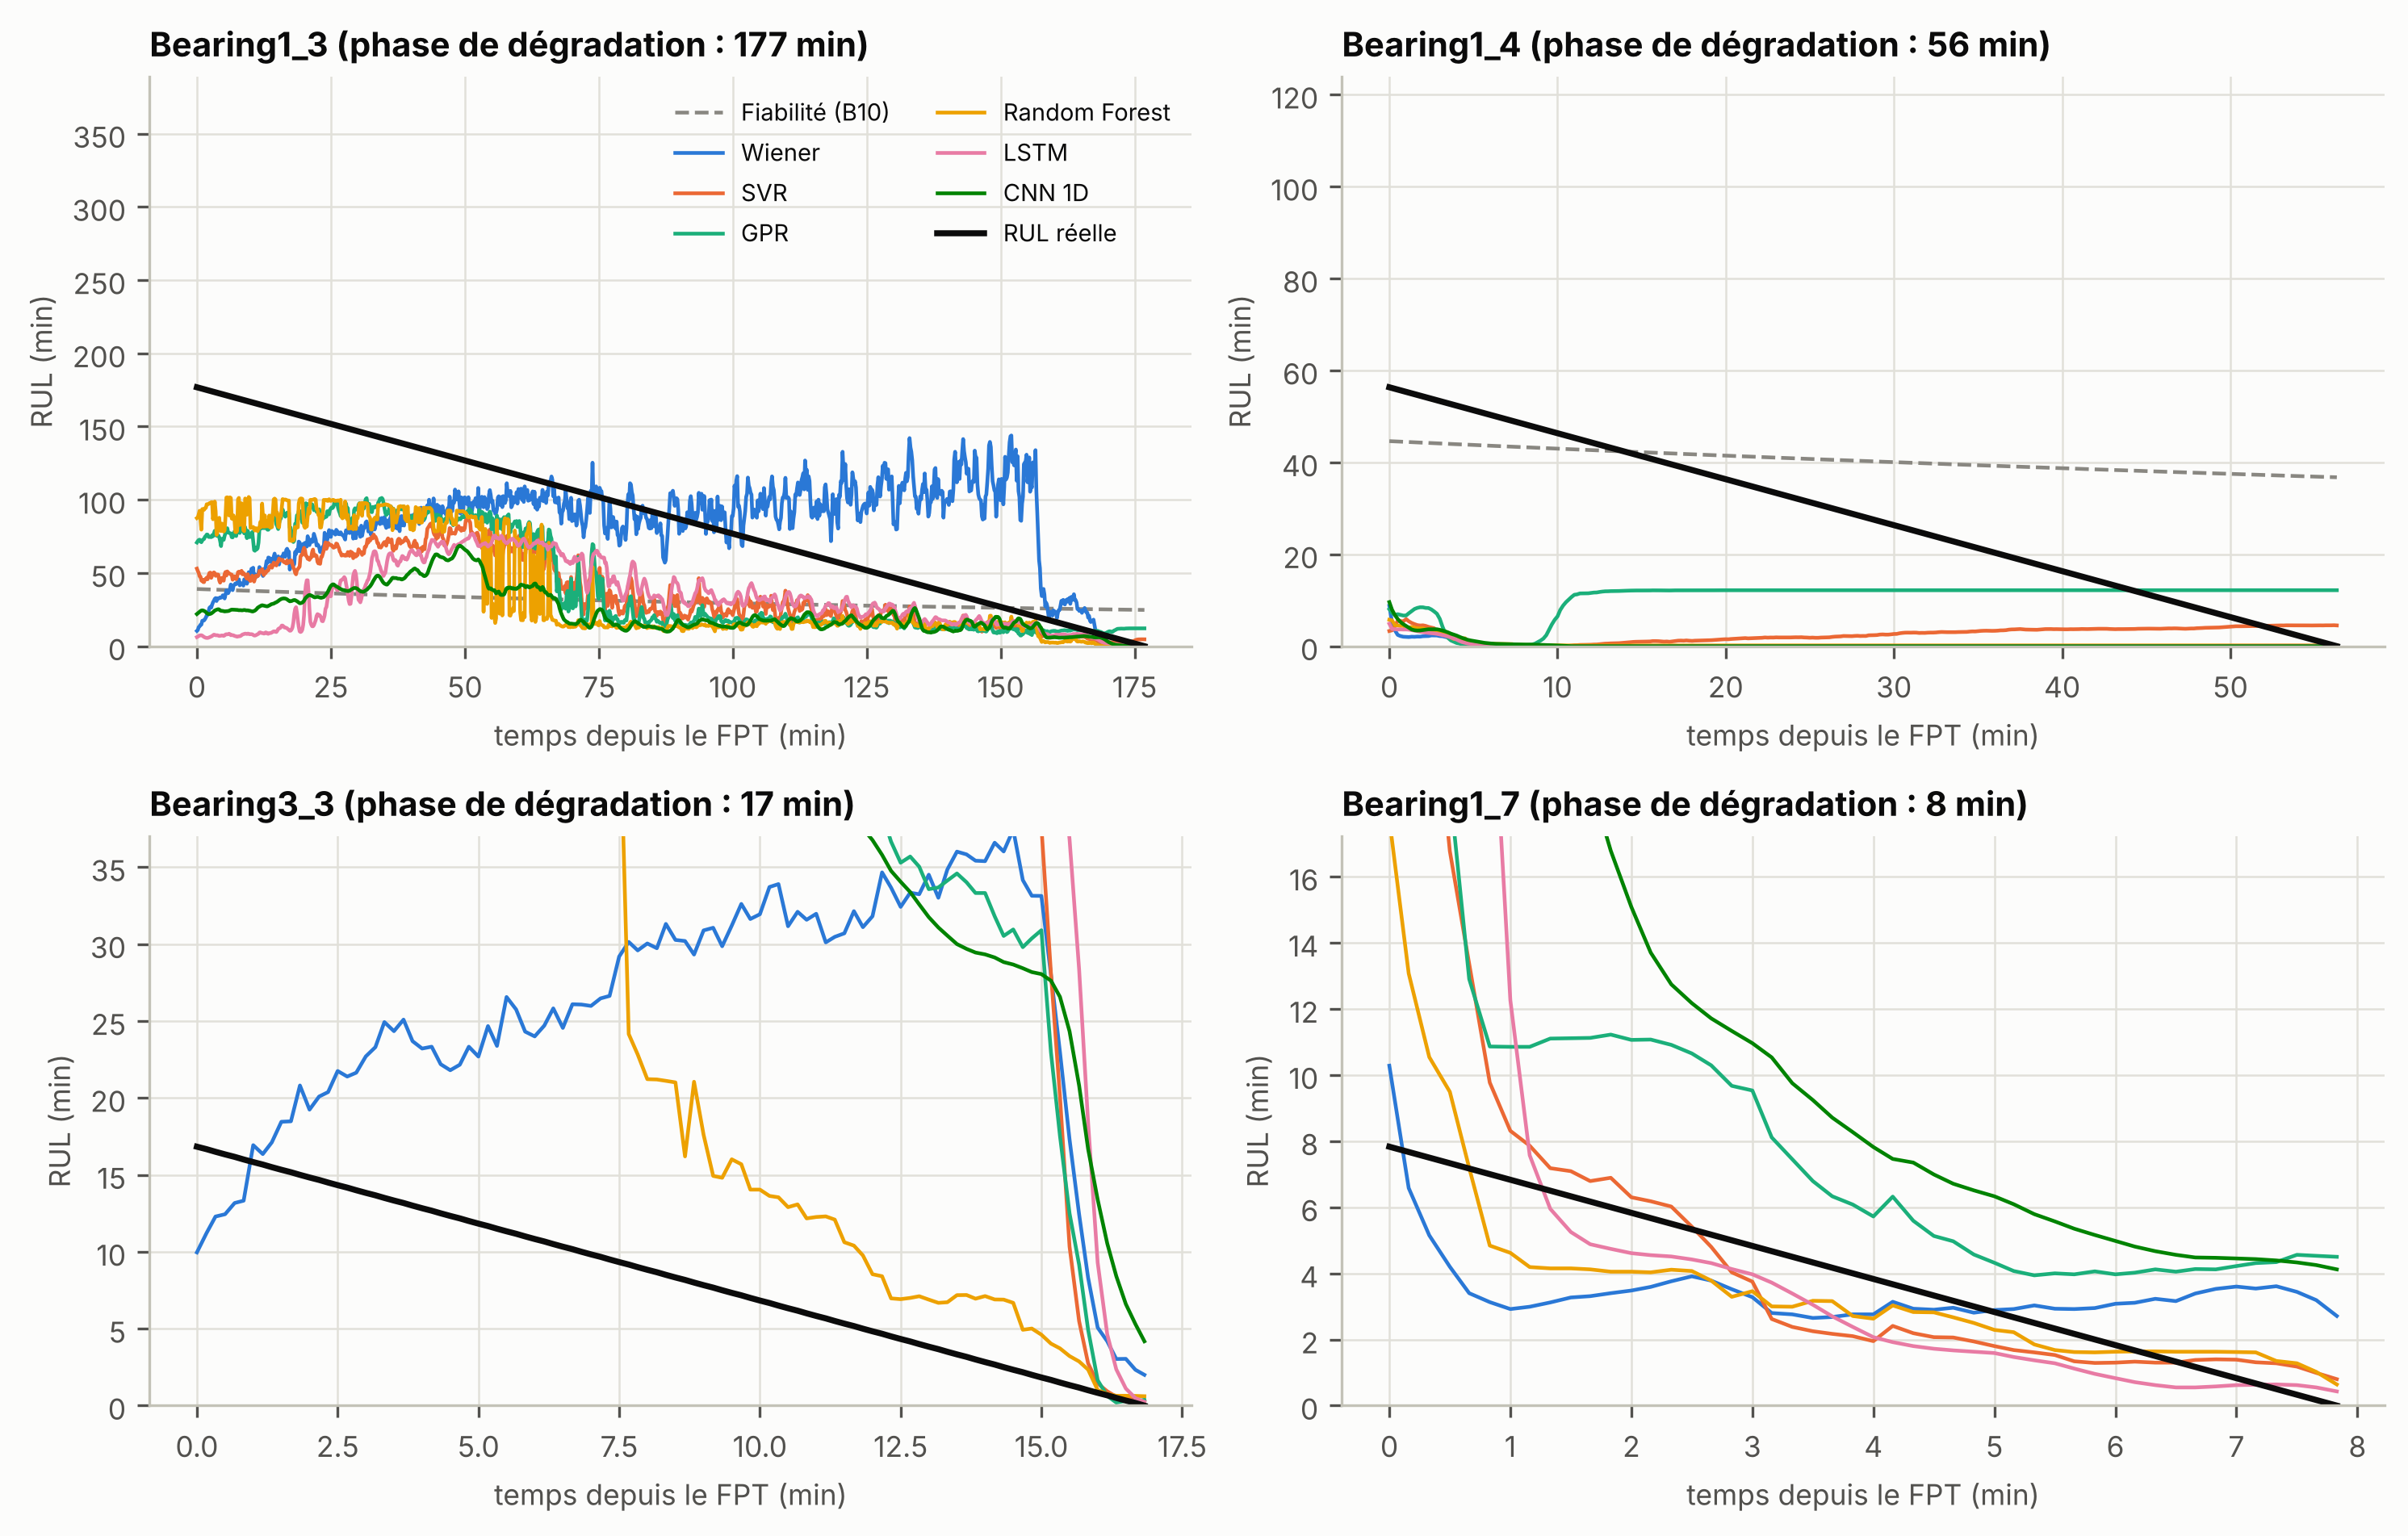
\includegraphics[width=0.86\linewidth]{figures/fig11_trajectoires_rul.png}
\caption[RUL prédite contre RUL réelle]{RUL prédite contre RUL réelle après le premier défaut, sur quatre roulements de test.}
\label{fig:trajectoires}
\end{figure}

\begin{figure}[H]
\centering
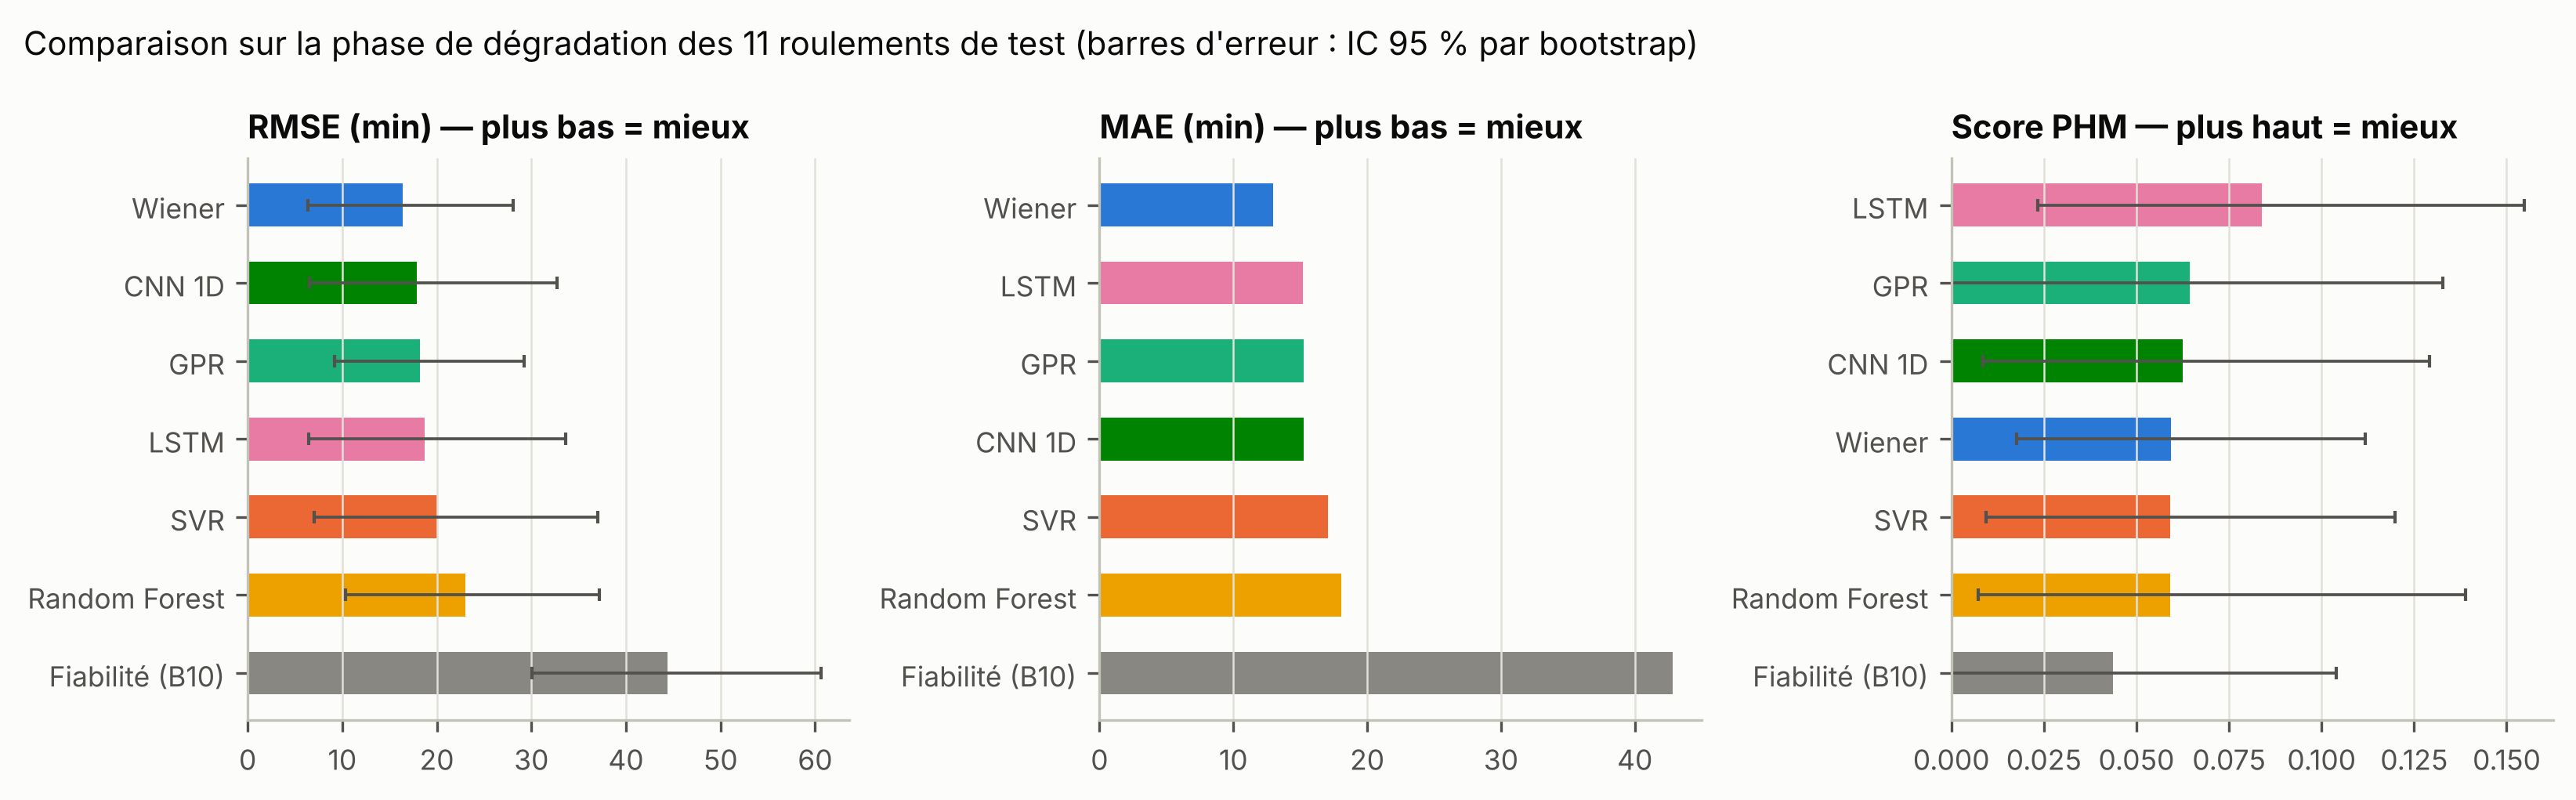
\includegraphics[width=\linewidth]{figures/fig13_comparaison_modeles.png}
\caption[Comparaison des méthodes avec intervalles]{RMSE, MAE et score PHM des sept méthodes (barres d'erreur : IC 95 \% par bootstrap).}
\label{fig:comparaison}
\end{figure}

\subsection{Les écarts sont-ils significatifs ?}
Les intervalles de confiance se chevauchent largement. Le test de Friedman sur les RMSE des 11 roulements donne $p = 0{,}022$ : au moins une méthode se distingue. Le test de Wilcoxon apparié montre que c'est la fiabilité seule : le Wiener la bat sur 9 roulements sur 11 ($p = 0{,}014$). Entre le Wiener et les autres méthodes fondées sur les capteurs, les écarts ne sont pas significatifs ($p$ de 0,21 à 0,70) : \textbf{11 roulements de test ne suffisent pas à les départager}.

\subsection{Benchmark multicritère}
Une méthode ne se juge pas seulement sur sa précision. Le tableau~\ref{tab:benchmark} ajoute la sécurité (prédire trop tard), l'incertitude, l'explicabilité et le coût de calcul.

\begin{table}[H]
\centering\small
\begin{tabular}{lccccc}
\toprule
Méthode & Précision & Sécurité & Intervalle d'incertitude & Explicabilité & Calcul \\
\midrule
Fiabilité (B10) & -- & -- & population & ++ & ++ \\
Wiener & ++ & + & oui & ++ & ++ \\
SVR & + & + & non & -- & + \\
GPR & + & + & possible & -- & + \\
Forêt aléatoire & 0 & + & non & + & + \\
LSTM & + & ++ & non & -- & -- \\
CNN 1D & + & + & non & -- & -- \\
\bottomrule
\end{tabular}
\caption[Benchmark multicritère]{Benchmark multicritère (++ très bon, + bon, 0 moyen, -- faible).}
\label{tab:benchmark}
\end{table}

\subsection{Covariables dans les modèles d'apprentissage}
Nous avons aussi ajouté la charge et la vitesse comme entrées des modèles d'apprentissage automatique (tableau~\ref{tab:covml}). Le GPR progresse sur tous les critères ; le SVR gagne en score mais perd en RMSE ; la forêt aléatoire change peu. Avec seulement 2 roulements d'apprentissage par condition, l'effet reste fragile.

\begin{table}[H]
\centering\small
\begin{tabular}{lcccccc}
\toprule
& \multicolumn{2}{c}{RMSE (min)} & \multicolumn{2}{c}{Score PHM} & \multicolumn{2}{c}{Score challenge} \\
Méthode & sans & avec & sans & avec & sans & avec \\
\midrule
SVR & 20,0 & 22,2 & 0,059 & 0,108 & 0,175 & 0,237 \\
GPR & 18,3 & 17,3 & 0,064 & 0,074 & 0,171 & 0,242 \\
Forêt aléatoire & 23,1 & 22,5 & 0,059 & 0,056 & 0,169 & 0,169 \\
\bottomrule
\end{tabular}
\caption[Covariables dans les modèles d'apprentissage]{Effet des covariables charge et vitesse sur les modèles d'apprentissage (recalcul dans les mêmes conditions).}
\label{tab:covml}
\end{table}

\section{Validation sur données simulées}

Sur des données réelles, on ne connaît jamais toute la vérité. Nous avons donc testé deux méthodes sur des données simulées où la réponse est connue (figure~\ref{fig:simulees}).

\textbf{Loi de Weibull.} On tire des durées de vie dans une Weibull connue ($\beta = 1{,}85$), avec le même plan d'essai que PRONOSTIA (6 essais complets, 11 censurés aux mêmes âges), puis on réestime $\beta$, 400 fois. Avec 17 roulements, $\beta$ estimé va de 1,36 à 3,34 dans 90 \% des cas, avec une légère surestimation en moyenne (2,15) ; avec 204 roulements, il va de 1,66 à 2,11. La méthode est juste, mais \textbf{17 roulements, c'est peu}.

\textbf{Processus de Wiener.} Quand les trajectoires suivent le modèle, l'intervalle à 90 \% contient bien 92 \% des vraies RUL : la méthode est correcte. Un HI qui stagne puis accélère ne la gêne presque pas (92 \%). En revanche, si le seuil de défaillance varie autant que sur les roulements de test (écart-type 1,57 au lieu de 0,63 à l'apprentissage), la couverture tombe à 63 \%, proche des 54 \% observés sur les vraies données. \textbf{Le problème vient du seuil, appris sur 6 roulements seulement, pas du modèle.} D'ailleurs, sans l'incertitude sur le seuil, la couverture réelle tombe à 31 \%.

\begin{figure}[H]
\centering
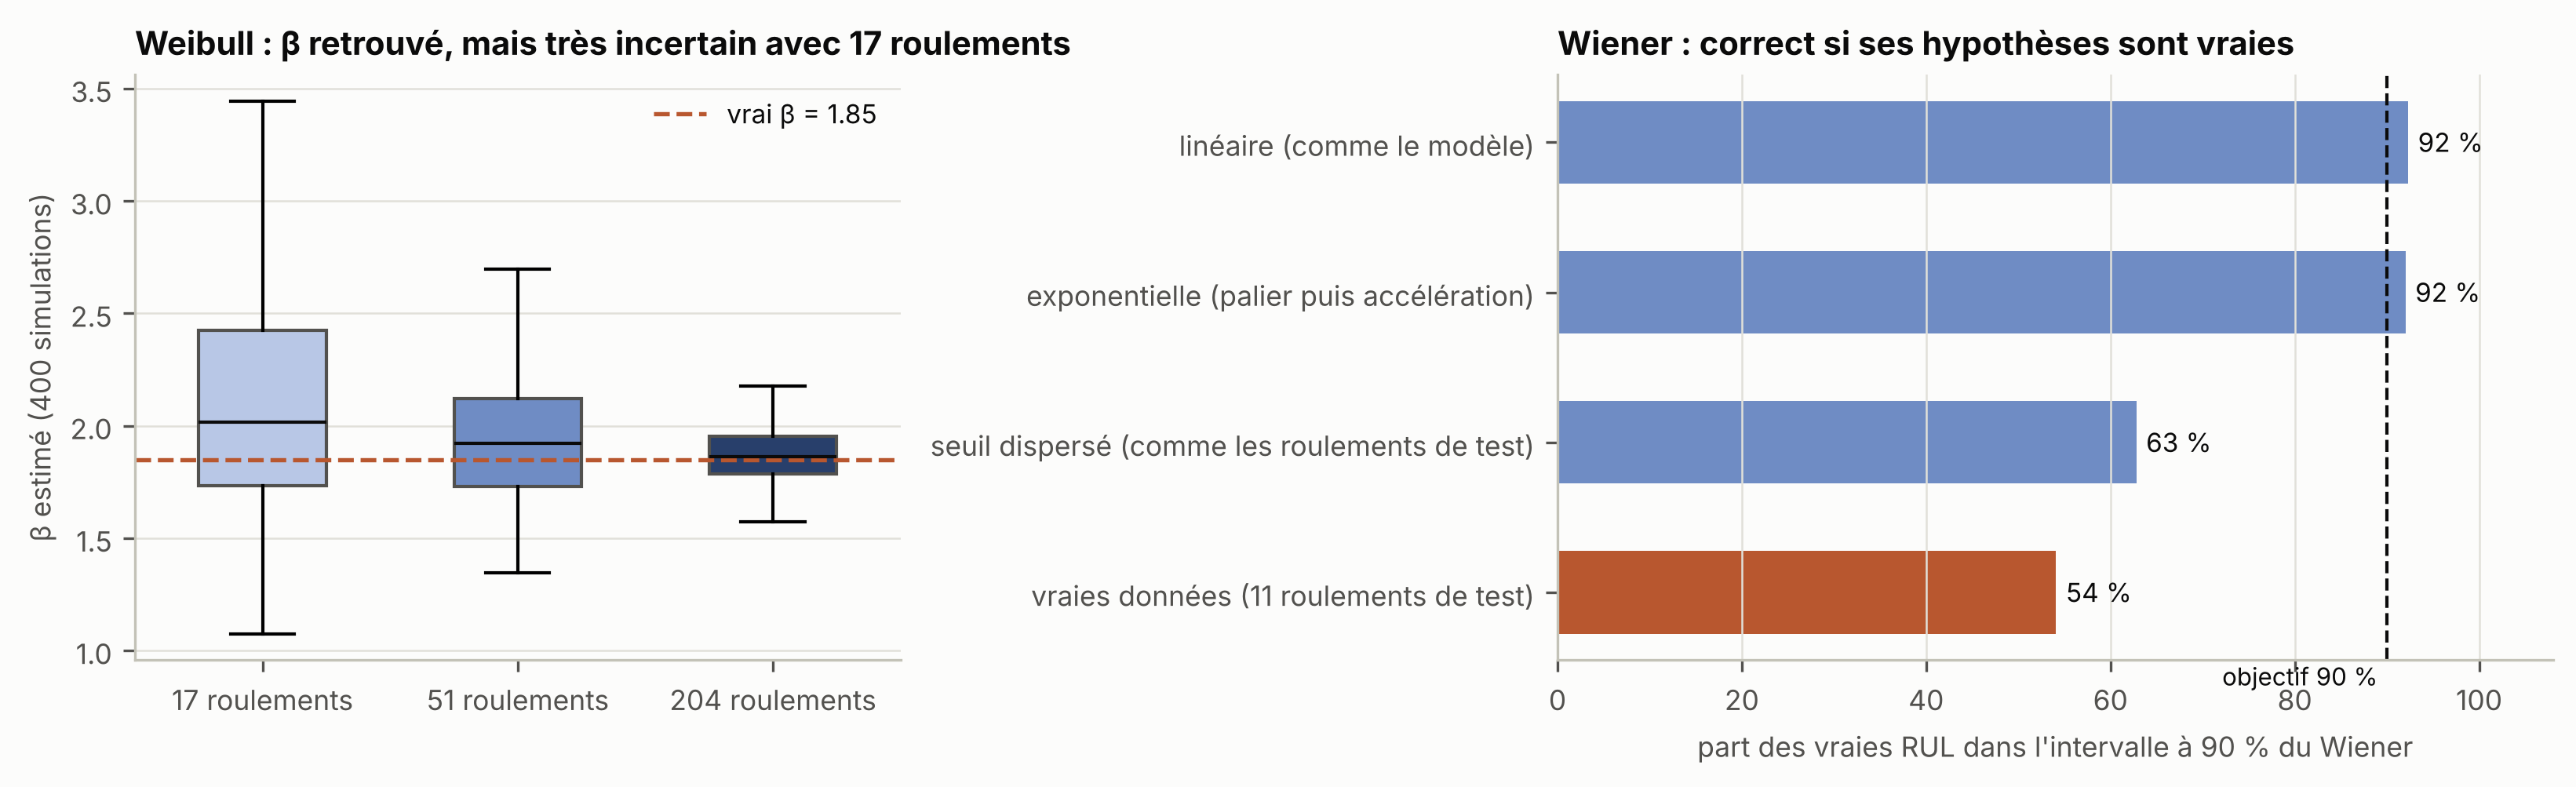
\includegraphics[width=\linewidth]{figures/fig20_donnees_simulees.png}
\caption[Validation sur données simulées]{Validation sur données simulées : estimation de $\beta$ selon le nombre de roulements, et couverture de l'intervalle du Wiener.}
\label{fig:simulees}
\end{figure}

\section{Explicabilité (XAI)}

Pour savoir sur quoi les modèles s'appuient, nous mélangeons au hasard une entrée et regardons de combien l'erreur augmente \cite{breiman2001}. La figure~\ref{fig:xai} montre que les trois modèles utilisent surtout les \textbf{énergies de bandes de fréquence}, et pas seulement le temps écoulé depuis le défaut : ils lisent vraiment l'état du roulement. Les bandes de 1,6 à 9,6 kHz dominent, là où résonnent les chocs d'un défaut. Le processus de Wiener, lui, est explicable par construction : une pente, un seuil, un bruit.

\begin{figure}[H]
\centering
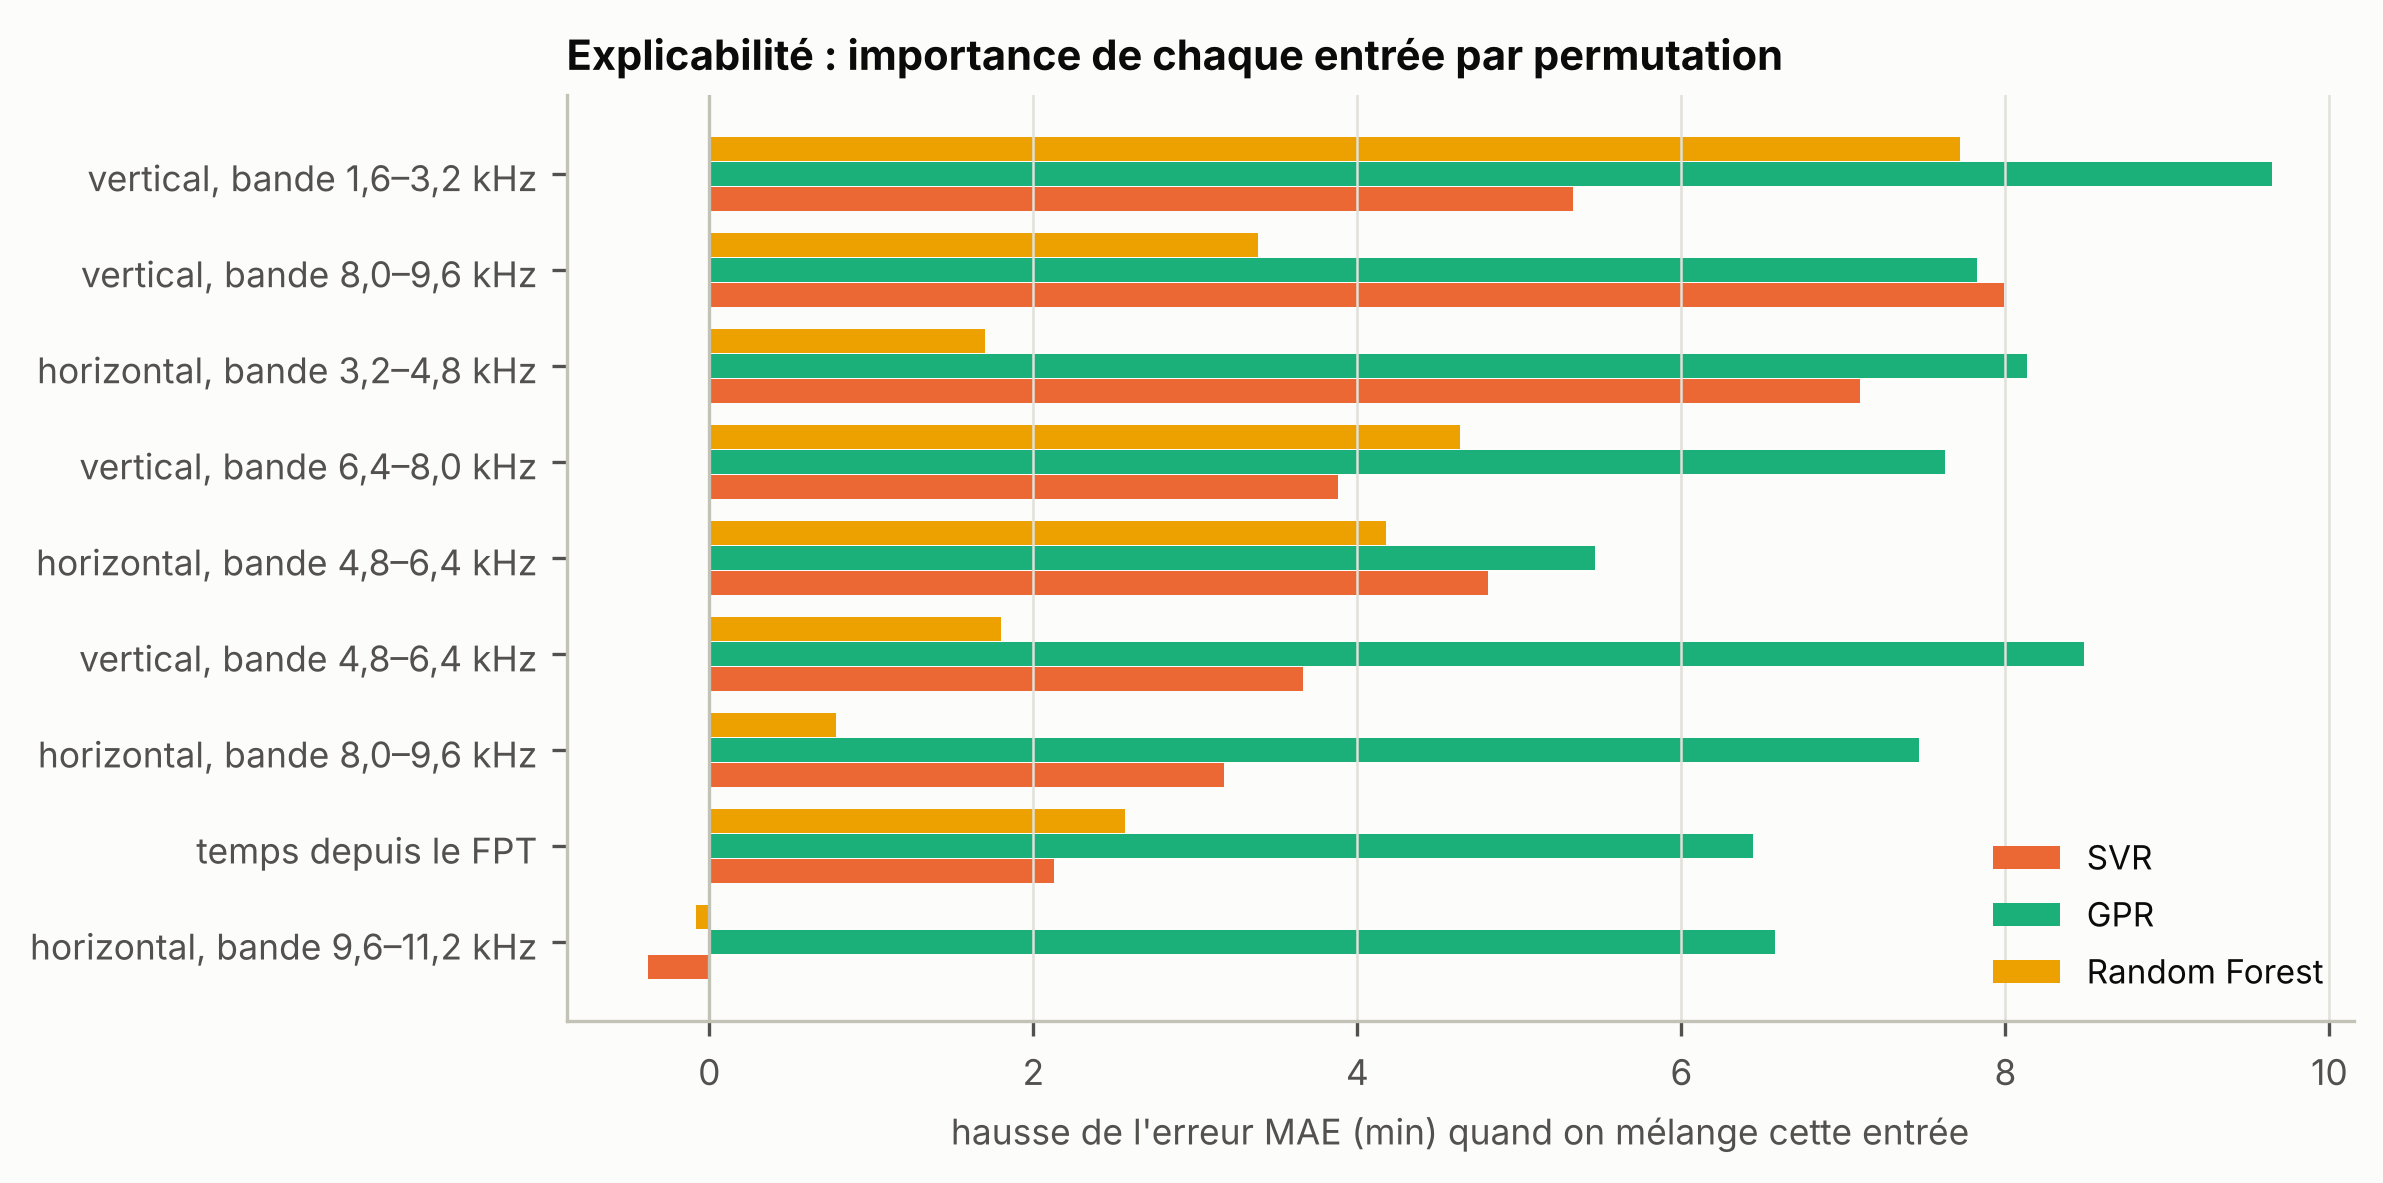
\includegraphics[width=0.72\linewidth]{figures/fig21_xai.png}
\caption[Explicabilité : importance des entrées]{Importance de chaque entrée par permutation, pour le SVR, le GPR et la forêt aléatoire.}
\label{fig:xai}
\end{figure}

\section{Restitution dans un tableau de bord}

Tous les résultats sont présentés dans un tableau de bord interactif en sept pages (figure~\ref{fig:dashboard}) : vue d'ensemble, données et fiabilité, santé et premier défaut, pronostic de la RUL, comparaison des méthodes, décision et économie, tests et validation. Le thème est sombre (noir et bleu), chaque page a sa nuance de bleu, et la page économique permet de changer les coûts en direct.

\begin{figure}[H]
\centering
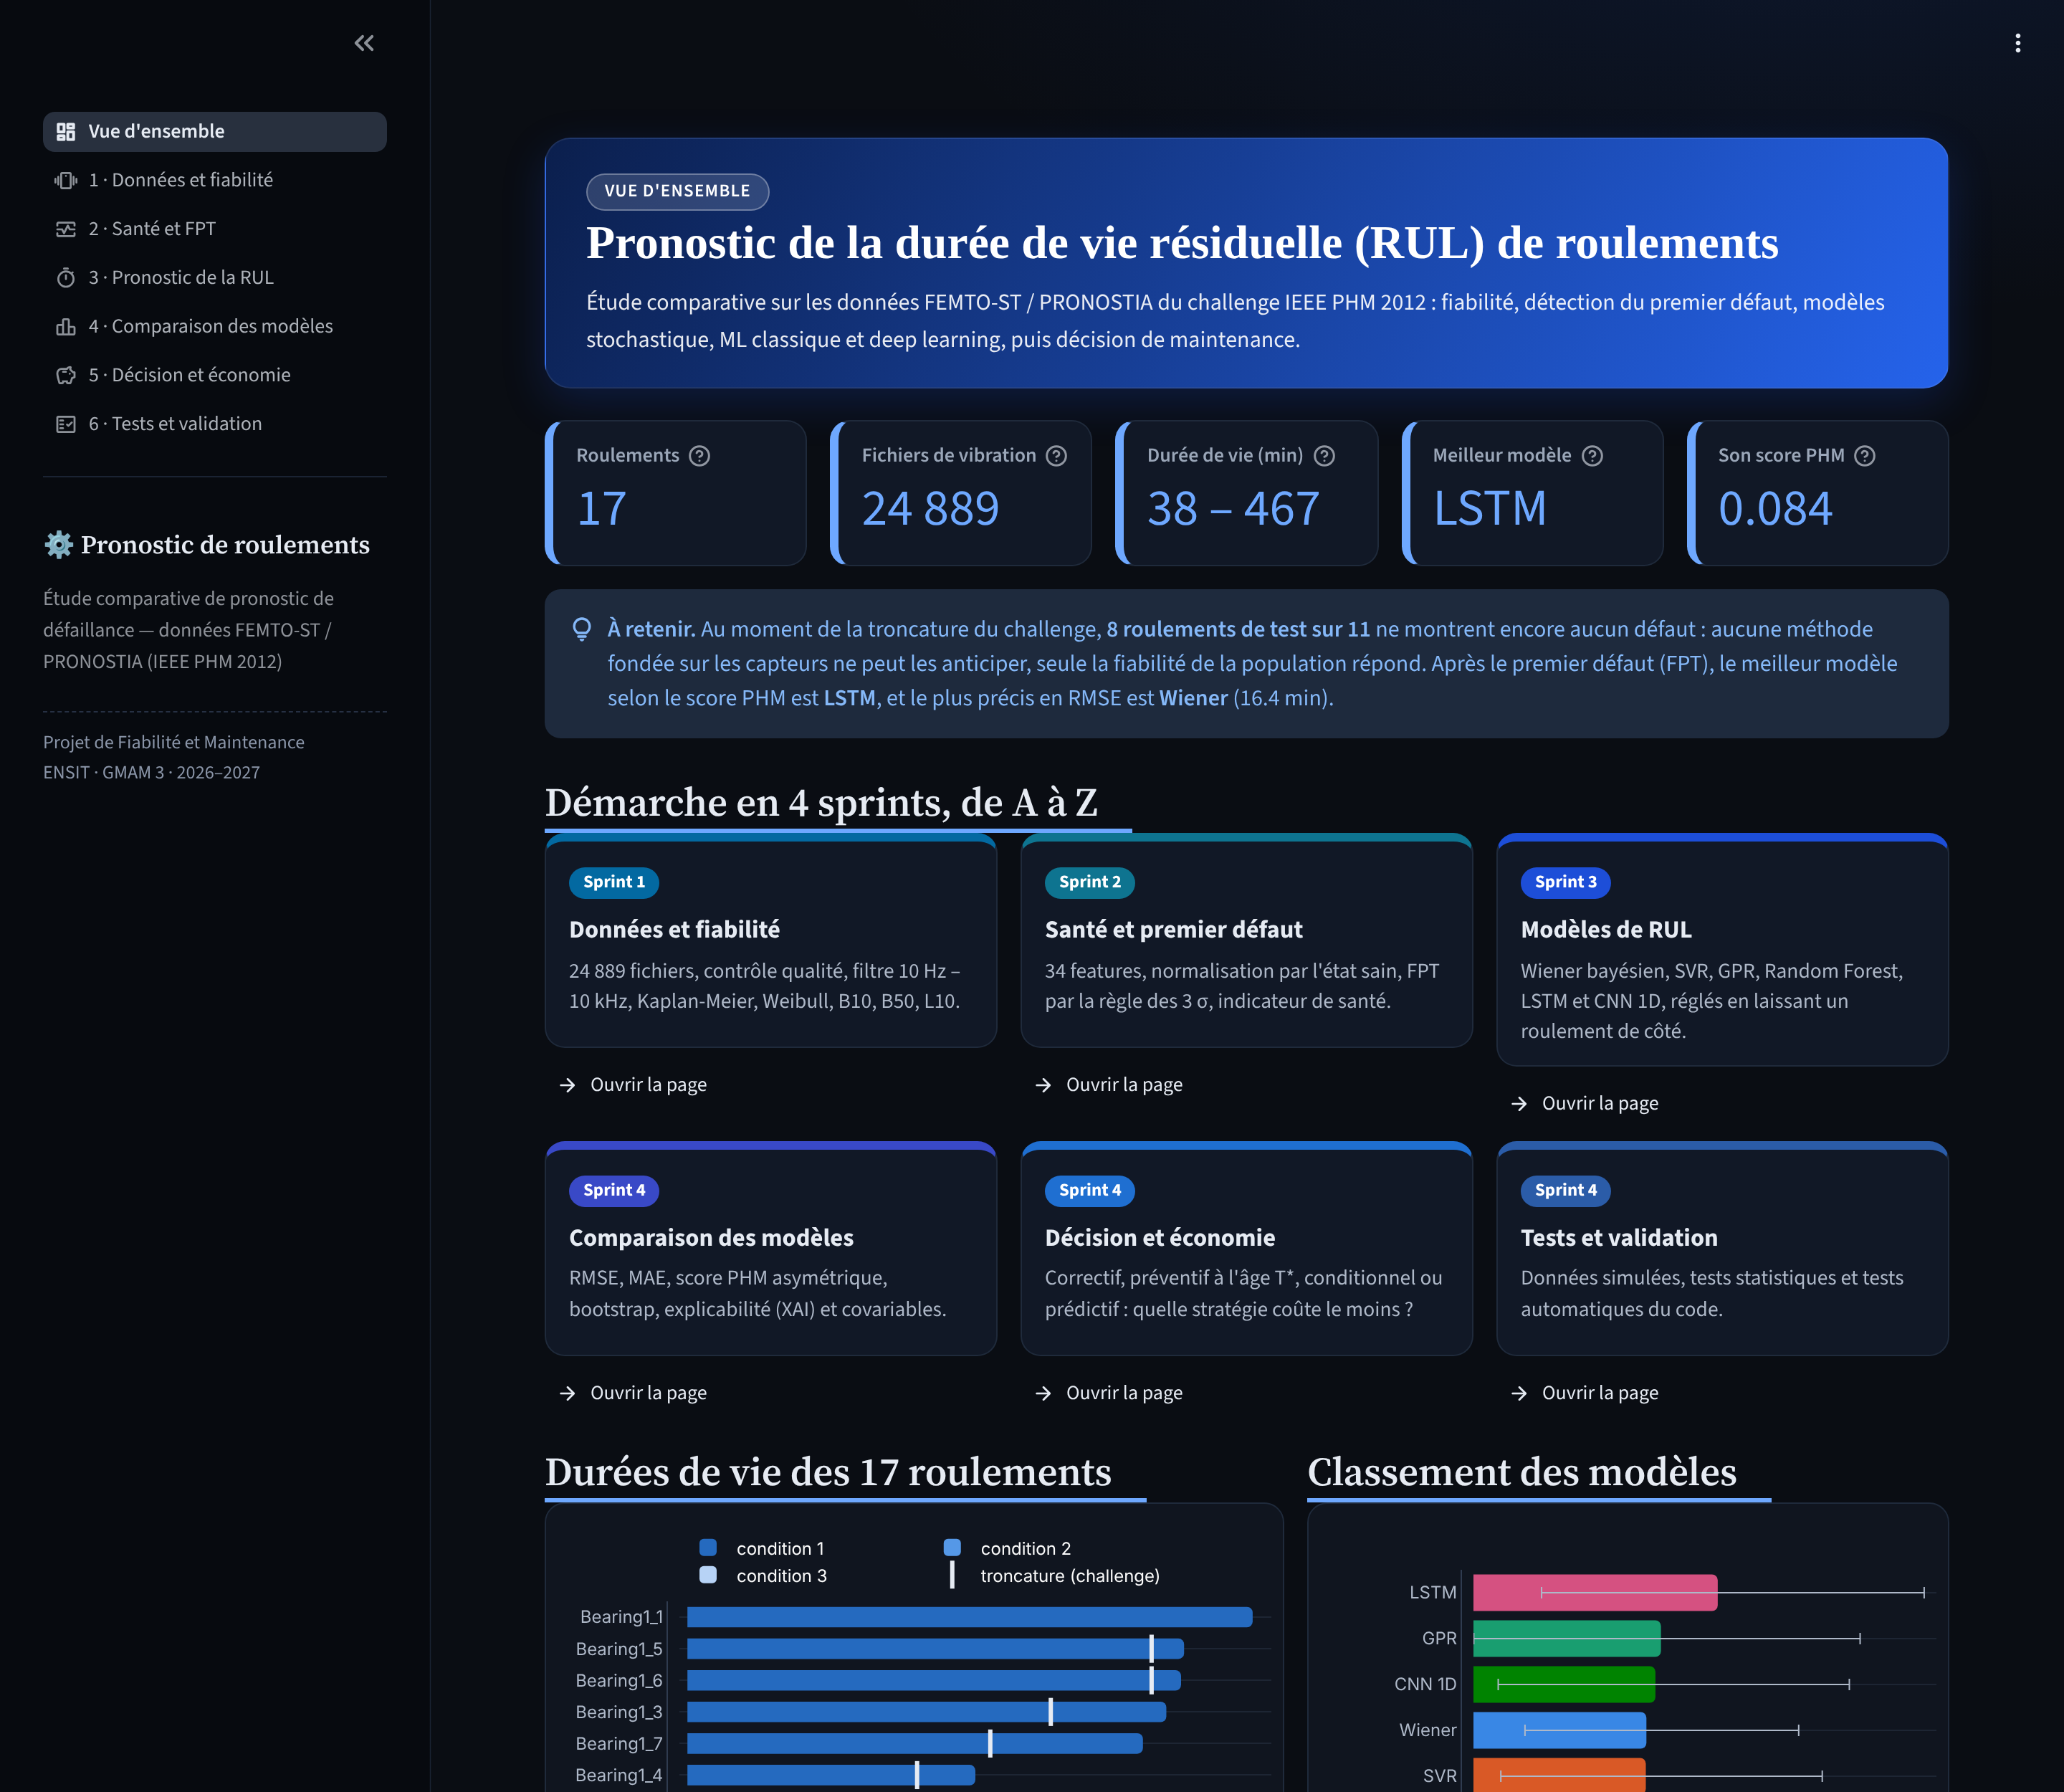
\includegraphics[width=0.7\linewidth]{figures/dashboard_accueil.png}
\caption[Page d'accueil du tableau de bord]{Page d'accueil du tableau de bord (Streamlit) : chiffres clés, démarche et classement des méthodes.}
\label{fig:dashboard}
\end{figure}

\chapconclusion
Après le premier défaut, les capteurs améliorent nettement la prédiction : le Wiener est le plus précis et le LSTM le plus prudent, mais les écarts entre méthodes ne sont pas significatifs avec 11 roulements. Les données simulées montrent que les méthodes sont correctes et que la principale faiblesse vient du seuil de défaillance, appris sur trop peu de roulements.

\chapter{Décision de maintenance, économie et perspectives}

\chapintro
Une bonne prédiction ne sert que si elle aide à décider. Ce chapitre transforme les prédictions en stratégies de maintenance, compare leur coût, résume les indicateurs clés du projet et propose des pistes d'amélioration.

\section{Hypothèses de l'analyse économique}

Le jeu de données ne contient aucun coût : nous utilisons les hypothèses du tableau~\ref{tab:hypotheses}, exprimées en unités relatives (1 u = le coût d'un remplacement planifié, par exemple 1 000 DT). Elles sont modifiables en direct dans le tableau de bord, et l'étude de sensibilité ci-dessous montre leur effet.

\begin{table}[H]
\centering\small
\begin{tabularx}{\linewidth}{lcY}
\toprule
Paramètre & Valeur & Signification \\
\midrule
Coût d'un remplacement planifié $C_p$ & 1 u & pièce et main-d'œuvre, intervention prévue \\
Coût d'une panne $C_c$ & 5 u & intervention en urgence, arrêt de production, dégâts \\
Coût d'une fausse alarme & 0,1 u & une inspection pour rien \\
Délai d'intervention & 2 min & temps entre la décision et le remplacement (échelle de l'essai accéléré) \\
Seuil de décision $s$ & 10 min & on remplace quand la RUL prédite passe sous $s$ \\
\bottomrule
\end{tabularx}
\caption[Hypothèses de l'analyse économique]{Hypothèses de l'analyse économique.}
\label{tab:hypotheses}
\end{table}

\section{Optimisation de la maintenance préventive}

Avec la loi de Weibull, le coût par heure $C(T)$ d'un remplacement à l'âge $T$ est minimal pour $\boldsymbol{T^* = 224}$ \textbf{min} (figure~\ref{fig:economie}, à gauche) : on économise 23 \% par rapport au tout correctif, en théorie. Ce gain existe parce que $\beta > 1$ : un roulement vieux casse plus souvent qu'un neuf. Le tableau~\ref{tab:rapport} montre que l'âge optimal et le gain dépendent beaucoup du rapport $C_c/C_p$ : si une panne coûte à peine plus qu'un remplacement, le préventif ne sert à rien.

\begin{table}[H]
\centering\small
\begin{tabular}{lcccccc}
\toprule
Rapport $C_c / C_p$ & 1,5 & 2 & 3 & 5 & 7 & 10 \\
\midrule
Âge optimal $T^*$ (min) & 858 & 520 & 336 & 224 & 179 & 143 \\
Gain théorique / correctif & 0 \% & 2 \% & 10 \% & 23 \% & 32 \% & 41 \% \\
\bottomrule
\end{tabular}
\caption[Âge optimal selon le rapport des coûts]{Sensibilité de l'âge optimal au rapport des coûts.}
\label{tab:rapport}
\end{table}

\section{Comparaison des stratégies}

Nous rejouons maintenant la vraie vie des 11 roulements de test avec chaque stratégie (figure~\ref{fig:economie}, à droite, et tableau~\ref{tab:strategies-cout}).

\begin{figure}[H]
\centering
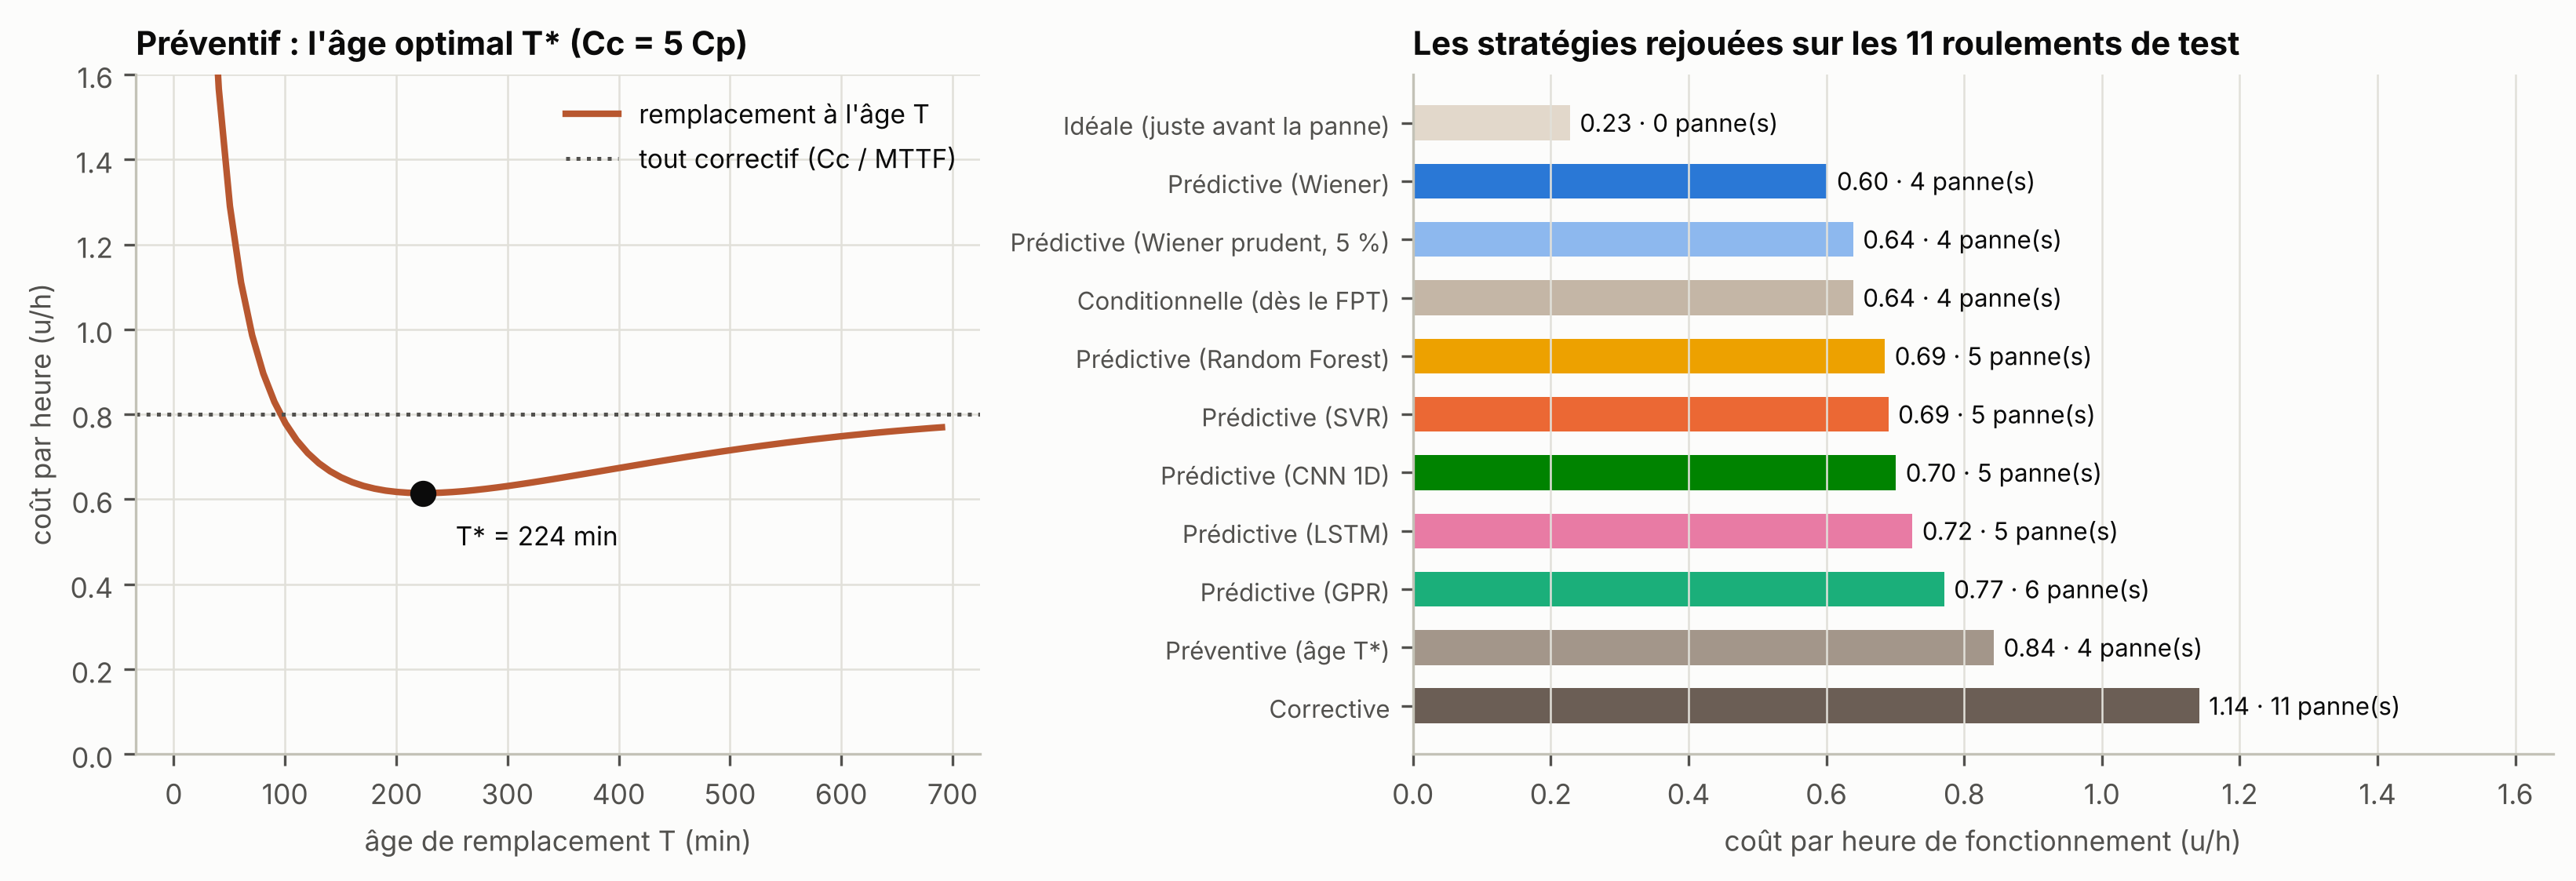
\includegraphics[width=\linewidth]{figures/fig22_economie.png}
\caption[Âge optimal et coût des stratégies]{À gauche : coût par heure d'un remplacement à l'âge $T$ et âge optimal $T^*$. À droite : coût par heure de chaque stratégie, rejouée sur les 11 roulements de test.}
\label{fig:economie}
\end{figure}

\begin{table}[H]
\centering\small
\begin{tabular}{lcccc}
\toprule
Stratégie & Coût (u/h) & Pannes (sur 11) & Vie gaspillée & Gain / correctif \\
\midrule
Corrective & 1,14 & 11 & 0 min & — \\
Préventive à l'âge $T^*$ & 0,84 & 4 & 139 min & 26 \% \\
Conditionnelle (dès le défaut) & 0,64 & 4 & 38 min & 44 \% \\
\textbf{Prédictive (Wiener)} & \textbf{0,60} & 4 & 14 min & \textbf{47 \%} \\
Prédictive (Wiener prudent, 5 \%) & 0,64 & 4 & 38 min & 44 \% \\
Prédictive (forêt aléatoire) & 0,68 & 5 & 15 min & 40 \% \\
Prédictive (SVR) & 0,69 & 5 & 18 min & 40 \% \\
Prédictive (CNN 1D) & 0,70 & 5 & 26 min & 39 \% \\
Prédictive (LSTM) & 0,73 & 5 & 41 min & 36 \% \\
Prédictive (GPR) & 0,77 & 6 & 18 min & 32 \% \\
Idéale (juste avant la panne) & 0,23 & 0 & 0 min & 80 \% \\
\bottomrule
\end{tabular}
\caption[Bilan économique des stratégies]{Bilan économique des stratégies sur les 11 roulements de test (vie gaspillée : moyenne sur les roulements remplacés avant la panne).}
\label{tab:strategies-cout}
\end{table}

Trois enseignements :
\begin{itemize}
  \item \textbf{Surveiller paie} : les stratégies conditionnelle et prédictives divisent presque le coût par deux par rapport au correctif, et font mieux que le préventif, qui jette en moyenne 139 min de vie par roulement.
  \item \textbf{La prédiction de la RUL apporte un gain de plus} : le Wiener utilise mieux la vie restante (14 min gaspillées au lieu de 38) sans ajouter de panne. C'est la meilleure stratégie réaliste (gain de 47 \%).
  \item \textbf{Les 4 pannes restantes sont inévitables avec des capteurs} : sur Bearing2\_3, Bearing2\_4, Bearing2\_6 et Bearing2\_7, le défaut apparaît 2 min ou moins avant la casse, ce qui ne laisse pas le temps d'intervenir. Le délai d'alerte doit être plus long que le délai d'intervention.
\end{itemize}
Le seuil $s$ se règle comme un hyperparamètre : trop petit, on intervient trop tard ; trop grand, on remplace dès l'alarme.

\section{Indicateurs clés (KPIs) du projet}

Le tableau~\ref{tab:kpis} rassemble les indicateurs clés, de la fiabilité jusqu'au coût.

\begin{table}[H]
\centering\small
\begin{tabularx}{\linewidth}{llY}
\toprule
Domaine & Indicateur & Valeur \\
\midrule
\multirow{3}{*}{Fiabilité} & MTTF & 375 min \\
& B10 / B50 & 125 min [78 ; 234] / 346 min [219 ; 573] \\
& Taux de défaillance à 300 min & 0,20 défaillance par heure \\
\midrule
\multirow{3}{*}{Détection} & Délai d'alerte médian (premier défaut → panne) & 7,8 min \\
& Fausses alarmes annulées & 14 (sur 8 roulements parmi 17) \\
& Tests dégradés à la troncature & 3 sur 11 \\
\midrule
\multirow{3}{*}{Pronostic} & Meilleure RMSE & 16,4 min (Wiener) \\
& Meilleur score PHM & 0,084 (LSTM) \\
& Couverture de l'intervalle à 90 \% & 54 \% (Wiener) \\
\midrule
\multirow{2}{*}{Économie} & Gain de la meilleure stratégie & $-47$ \% de coût par heure (Wiener prédictif) \\
& Pannes évitées & 7 sur 11 (64 \%) \\
\bottomrule
\end{tabularx}
\caption[Indicateurs clés de performance (KPIs)]{Indicateurs clés de performance du projet.}
\label{tab:kpis}
\end{table}

\section{Interprétation industrielle et limites}

En usine, la démarche s'utiliserait en deux temps : la fiabilité de la population fixe un plan de base (inspection, stock de pièces de rechange), puis la surveillance vibratoire déclenche l'intervention roulement par roulement. Nos résultats ont cependant des limites :
\begin{itemize}
  \item \textbf{peu de données} : 6 roulements d'apprentissage et des durées de vie de 38 à 467 min, même sous une même condition ;
  \item \textbf{défaillances brutales} : pour la plupart des roulements de test, le défaut détectable dure moins de 17 min ;
  \item \textbf{intervalles trop étroits} : l'intervalle du Wiener ne contient la vraie RUL que dans 54 \% des cas, à cause du seuil de défaillance ;
  \item \textbf{coûts et temps illustratifs} : l'essai est accéléré, et les coûts sont des hypothèses à remplacer par ceux de l'usine.
\end{itemize}

\section{Perspectives}

\begin{itemize}
  \item \textbf{Mieux modéliser la dégradation} : modèle exponentiel ou filtre particulaire, et un seuil de défaillance appris par condition opératoire.
  \item \textbf{Calibrer l'incertitude} : élargir les intervalles à partir des erreurs observées, par exemple avec la prédiction conforme, pour atteindre vraiment 90 \%.
  \item \textbf{Autres réseaux} : GRU et TCN, apprentissage par transfert d'une condition à l'autre \cite{dhungana2025}.
  \item \textbf{Plus de covariables} : température du roulement (mesurée sur certains essais PRONOSTIA), lubrification, profil de charge réel.
  \item \textbf{Explicabilité plus fine} : valeurs de Shapley pour expliquer chaque prédiction, pas seulement le modèle.
  \item \textbf{Déploiement} : calcul en temps réel près de la machine et alertes envoyées à l'équipe de maintenance.
\end{itemize}

\chapconclusion
La surveillance vibratoire, associée à une prédiction de la RUL, réduit le coût de maintenance d'environ moitié dans notre étude, à condition que le défaut soit détecté assez tôt pour intervenir. Le processus de Wiener offre le meilleur compromis entre précision, simplicité et explicabilité.

\chapter*{Conclusion générale}
\addcontentsline{toc}{chapter}{Conclusion générale}
\frontmark{Conclusion générale}

Ce projet a suivi toute la démarche de la sûreté de fonctionnement sur des roulements réels, du fichier de vibration jusqu'à la décision de maintenance, en quatre sprints.

La \textbf{fiabilité de la population}, calculée en tenant compte des roulements censurés, suit une loi de Weibull de forme $\beta = 1{,}85$ : un roulement sur dix casse avant 125 min (B10) et la moitié avant 346 min (B50). Avec seulement 6 défaillances, ces valeurs restent incertaines, comme l'ont confirmé le bootstrap et les données simulées. La charge, ajoutée comme covariable, raccourcit nettement la durée de vie.

La \textbf{surveillance vibratoire} détecte le premier défaut en médiane 7,8 min avant la panne, avec une règle simple qui fonctionne en temps réel. Après ce défaut, toutes les méthodes fondées sur les capteurs prédisent bien mieux que la fiabilité seule. Le processus de Wiener bayésien est le plus précis (RMSE de 16,4 min) et le plus simple à expliquer ; le LSTM est le plus prudent. Avec 11 roulements de test, les écarts entre ces méthodes ne sont toutefois pas significatifs.

Sur le plan \textbf{économique}, rejouer la vie des roulements de test montre qu'une maintenance prédictive fondée sur le Wiener réduit le coût par heure de 47 \% par rapport au correctif, et fait mieux que le remplacement préventif à l'âge optimal. La limite principale est physique : quand le défaut apparaît moins de 2 min avant la casse, aucune méthode ne laisse le temps d'intervenir.

Les tests sur données simulées ont aussi montré d'où vient la principale faiblesse : le seuil de défaillance, appris sur trop peu de roulements, rend les intervalles d'incertitude trop étroits. Les prochaines étapes sont donc claires : plus d'essais, un seuil appris par condition, des intervalles calibrés, et d'autres variables comme la température.

Au-delà des chiffres, ce travail nous a appris qu'un bon pronostic ne vaut que par la décision qu'il permet, et qu'il faut toujours tester une méthode là où l'on connaît la réponse avant de lui faire confiance.

% Bibliographie au format IEEE, générée par BibTeX à partir de references.bib
% (fichier importable dans Zotero : Fichier > Importer).
\chapter*{Bibliographie}
\addcontentsline{toc}{chapter}{Bibliographie}
\frontmark{Bibliographie}
\begin{multicols}{2}
\footnotesize\setstretch{1.0}\sloppy
\begingroup
\renewcommand{\chapter}[2]{}% le titre « Bibliographie » est déjà imprimé
\bibliographystyle{ieeetr}
\bibliography{references}
\endgroup
\end{multicols}

\chapter*{Annexes}
\addcontentsline{toc}{chapter}{Annexes}
\frontmark{Annexes}

\section*{Annexe A -- Paramètres et hypothèses}

\begin{table}[H]
\centering\small
\begin{tabularx}{\linewidth}{lY}
\toprule
Élément & Valeur retenue \\
\midrule
État sain de référence & fichiers 31 à 150 (de 5 à 25 min) \\
Lissage & moyenne glissante sur 6 mesures (1 min), passé seulement \\
Premier défaut & 3 $\sigma$, 3 mesures consécutives, annulation après 5 min sous le seuil \\
Entrées des modèles & 8 énergies de bandes d'ondelettes et le temps depuis le premier défaut \\
Indicateur de santé & énergie de la bande 6,4--8,0 kHz (axe vertical), seuil $D = 3{,}34 \pm 0{,}63$ \\
Wiener & $\mu_0 = 0{,}281$ /min, $s_0 = 0{,}276$ /min, $\sigma = 0{,}245$, 2 000 tirages \\
SVR & $C = 1$, $\gamma = 0{,}1$, $\varepsilon = 0{,}05$ \\
GPR & noyau RBF + bruit blanc, longueur de départ 1,0 \\
Forêt aléatoire & 300 arbres, 50 \% des entrées par nœud, 5 exemples par feuille \\
LSTM / CNN 1D & 32 unités, fenêtre de 6 mesures / 16 filtres, fenêtre de 12 mesures \\
Économie & $C_p = 1$ u, $C_c = 5$ u, fausse alarme 0,1 u, délai 2 min, seuil 10 min \\
Graine aléatoire & 42 (tous les résultats se refont à l'identique) \\
\bottomrule
\end{tabularx}
\caption[Paramètres et hypothèses du projet]{Paramètres et hypothèses du projet.}
\label{tab:parametres}
\end{table}

\section*{Annexe B -- Code, tests et bibliographie}

\textbf{Organisation du code.} Le projet (Python, scikit-learn, lifelines, Keras) tient en quatre scripts, à lancer dans l'ordre :
\begin{itemize}[nosep,leftmargin=1.6em]
  \item \texttt{1\_extraire\_features.py} : des signaux bruts aux features ;
  \item \texttt{2\_lancer\_pipeline.py} : sprints 2 à 4 (santé, modèles, évaluation) ;
  \item \texttt{3\_figures\_rapport.py} : les figures du rapport ;
  \item \texttt{4\_analyses\_complementaires.py} : vraisemblance, covariables, XAI, économie.
\end{itemize}
Le dossier \texttt{src/} contient un module par étape, \texttt{dashboard/} le tableau de bord (\texttt{streamlit run dashboard/app.py}) et \texttt{tests/} les 29 tests automatiques (\texttt{python -m pytest}).

\textbf{Reproductibilité.} Chaque exécution enregistre la date, la durée et les versions des bibliothèques (\texttt{results/run\_info.json}) ; seuls les réseaux de neurones varient un peu d'un PC à l'autre.

\textbf{Bibliographie.} Les références, au format IEEE, sont dans \texttt{references.bib}, qui s'importe directement dans Zotero. Le connecteur Zotero du navigateur ajoute une référence depuis Google Scholar ou IEEE Xplore en un clic ; ses modules pour Word et Google Docs citent au même format.

\clearpage\pagestyle{empty}\thispagestyle{empty}
\addcontentsline{toc}{chapter}{Résumé}
\setstretch{1.05}\small

\noindent{\large\bfseries Résumé}\par\medskip

Ce rapport présente une étude comparative de pronostic de défaillance de roulements sur les données réelles du banc PRONOSTIA (FEMTO-ST, challenge IEEE PHM 2012). La fiabilité de la population, estimée par maximum de vraisemblance en tenant compte des roulements censurés, suit une loi de Weibull ($\beta$ = 1,85) : B10 = 125 min et B50 = 346 min, avec de larges intervalles de confiance. Un défaut est détecté par la règle des 3 $\sigma$ en médiane 7,8 min avant la panne, et un indicateur de santé est construit à partir d'énergies de bandes d'ondelettes. Sept méthodes de prédiction de la durée de vie résiduelle sont comparées : le processus de Wiener bayésien est le plus précis (RMSE de 16,4 min) et le LSTM le plus prudent. Des tests sur données simulées, des tests statistiques et une analyse d'explicabilité valident la démarche. Enfin, une maintenance prédictive fondée sur le Wiener réduit le coût par heure de 47 \% par rapport au correctif.

\textbf{Mots-clés :} fiabilité, loi de Weibull, vraisemblance, durée de vie résiduelle, processus de Wiener, apprentissage automatique, maintenance prédictive.

\par\medskip\noindent\rule{\linewidth}{0.4pt}\par\medskip
\begin{otherlanguage}{english}
\noindent{\large\bfseries Abstract}\par\medskip

This report presents a comparative study of bearing failure prognostics on the real PRONOSTIA dataset (FEMTO-ST, IEEE PHM 2012 challenge). The population reliability, estimated by maximum likelihood with right-censored bearings, follows a Weibull distribution ($\beta$ = 1.85): B10 = 125 min and B50 = 346 min, with wide confidence intervals. A first defect is detected by a 3-sigma rule a median of 7.8 min before failure, and a health indicator is built from wavelet band energies. Seven remaining useful life methods are compared: the Bayesian Wiener process is the most accurate (RMSE of 16.4 min) and the LSTM the most cautious. Tests on simulated data, statistical tests and an explainability analysis validate the approach. Finally, a predictive maintenance policy based on the Wiener model cuts the cost per hour by 47\% compared with corrective maintenance.

\textbf{Keywords:} reliability, Weibull distribution, likelihood, remaining useful life, Wiener process, machine learning, predictive maintenance.
\end{otherlanguage}

\par\medskip\noindent\rule{\linewidth}{0.4pt}\par\medskip
\resumearabe

\end{document}
